%% bare_jrnl_transmag.tex
%% V1.4b
%% 2015/08/26
%% by Michael Shell
%% see http://www.michaelshell.org/
%% for current contact information.
%%
%% This is a skeleton file demonstrating the use of IEEEtran.cls
%% (requires IEEEtran.cls version 1.8b or later) with an IEEE 
%% Transactions on Magnetics journal paper.
%%
%% Support sites:
%% http://www.michaelshell.org/tex/ieeetran/
%% http://www.ctan.org/pkg/ieeetran
%% and
%% http://www.ieee.org/

%%*************************************************************************
%% Legal Notice:
%% This code is offered as-is without any warranty either expressed or
%% implied; without even the implied warranty of MERCHANTABILITY or
%% FITNESS FOR A PARTICULAR PURPOSE! 
%% User assumes all risk.
%% In no event shall the IEEE or any contributor to this code be liable for
%% any damages or losses, including, but not limited to, incidental,
%% consequential, or any other damages, resulting from the use or misuse
%% of any information contained here.
%%
%% All comments are the opinions of their respective authors and are not
%% necessarily endorsed by the IEEE.
%%
%% This work is distributed under the LaTeX Project Public License (LPPL)
%% ( http://www.latex-project.org/ ) version 1.3, and may be freely used,
%% distributed and modified. A copy of the LPPL, version 1.3, is included
%% in the base LaTeX documentation of all distributions of LaTeX released
%% 2003/12/01 or later.
%% Retain all contribution notices and credits.
%% ** Modified files should be clearly indicated as such, including  **
%% ** renaming them and changing author support contact information. **
%%*************************************************************************


% *** Authors should verify (and, if needed, correct) their LaTeX system  ***
% *** with the testflow diagnostic prior to trusting their LaTeX platform ***
% *** with production work. The IEEE's font choices and paper sizes can   ***
% *** trigger bugs that do not appear when using other class files.       ***                          ***
% The testflow support page is at:
% http://www.michaelshell.org/tex/testflow/



\documentclass[journal,transmag]{IEEEtran}
%
% If IEEEtran.cls has not been installed into the LaTeX system files,
% manually specify the path to it like:
% \documentclass[journal]{../sty/IEEEtran}


\newcommand{\tabincell}[2]{\begin{tabular}{@{}#1@{}}#2\end{tabular}}
\usepackage{diagbox}
\usepackage{subfigure}
\usepackage[justification=centering]{caption} 
\usepackage{algorithm}
%\usepackage{algorithmic}
\usepackage{algpseudocode}
\usepackage{amsmath}
\usepackage{graphics}
\usepackage{epsfig}
\usepackage{float}
\usepackage{hyperref}
\usepackage{multirow}
\usepackage[marginal]{footmisc}
\renewcommand{\thefootnote}{}

\renewcommand{\algorithmicrequire}{\textbf{Require:}}



% Some very useful LaTeX packages include:
% (uncomment the ones you want to load)


% *** MISC UTILITY PACKAGES ***
%
%\usepackage{ifpdf}
% Heiko Oberdiek's ifpdf.sty is very useful if you need conditional
% compilation based on whether the output is pdf or dvi.
% usage:
% \ifpdf
%   % pdf code
% \else
%   % dvi code
% \fi
% The latest version of ifpdf.sty can be obtained from:
% http://www.ctan.org/pkg/ifpdf
% Also, note that IEEEtran.cls V1.7 and later provides a builtin
% \ifCLASSINFOpdf conditional that works the same way.
% When switching from latex to pdflatex and vice-versa, the compiler may
% have to be run twice to clear warning/error messages.






% *** CITATION PACKAGES ***
%
%\usepackage{cite}
% cite.sty was written by Donald Arseneau
% V1.6 and later of IEEEtran pre-defines the format of the cite.sty package
% \cite{} output to follow that of the IEEE. Loading the cite package will
% result in citation numbers being automatically sorted and properly
% "compressed/ranged". e.g., [1], [9], [2], [7], [5], [6] without using
% cite.sty will become [1], [2], [5]--[7], [9] using cite.sty. cite.sty's
% \cite will automatically add leading space, if needed. Use cite.sty's
% noadjust option (cite.sty V3.8 and later) if you want to turn this off
% such as if a citation ever needs to be enclosed in parenthesis.
% cite.sty is already installed on most LaTeX systems. Be sure and use
% version 5.0 (2009-03-20) and later if using hyperref.sty.
% The latest version can be obtained at:
% http://www.ctan.org/pkg/cite
% The documentation is contained in the cite.sty file itself.






% *** GRAPHICS RELATED PACKAGES ***
%
\ifCLASSINFOpdf
  % \usepackage[pdftex]{graphicx}
  % declare the path(s) where your graphic files are
  % \graphicspath{{../pdf/}{../jpeg/}}
  % and their extensions so you won't have to specify these with
  % every instance of \includegraphics
  % \DeclareGraphicsExtensions{.pdf,.jpeg,.png}
\else
  % or other class option (dvipsone, dvipdf, if not using dvips). graphicx
  % will default to the driver specified in the system graphics.cfg if no
  % driver is specified.
  % \usepackage[dvips]{graphicx}
  % declare the path(s) where your graphic files are
  % \graphicspath{{../eps/}}
  % and their extensions so you won't have to specify these with
  % every instance of \includegraphics
  % \DeclareGraphicsExtensions{.eps}
\fi
% graphicx was written by David Carlisle and Sebastian Rahtz. It is
% required if you want graphics, photos, etc. graphicx.sty is already
% installed on most LaTeX systems. The latest version and documentation
% can be obtained at: 
% http://www.ctan.org/pkg/graphicx
% Another good source of documentation is "Using Imported Graphics in
% LaTeX2e" by Keith Reckdahl which can be found at:
% http://www.ctan.org/pkg/epslatex
%
% latex, and pdflatex in dvi mode, support graphics in encapsulated
% postscript (.eps) format. pdflatex in pdf mode supports graphics
% in .pdf, .jpeg, .png and .mps (metapost) formats. Users should ensure
% that all non-photo figures use a vector format (.eps, .pdf, .mps) and
% not a bitmapped formats (.jpeg, .png). The IEEE frowns on bitmapped formats
% which can result in "jaggedy"/blurry rendering of lines and letters as
% well as large increases in file sizes.
%
% You can find documentation about the pdfTeX application at:
% http://www.tug.org/applications/pdftex




% *** MATH PACKAGES ***
%
%\usepackage{amsmath}
% A popular package from the American Mathematical Society that provides
% many useful and powerful commands for dealing with mathematics.
%
% Note that the amsmath package sets \interdisplaylinepenalty to 10000
% thus preventing page breaks from occurring within multiline equations. Use:
%\interdisplaylinepenalty=2500
% after loading amsmath to restore such page breaks as IEEEtran.cls normally
% does. amsmath.sty is already installed on most LaTeX systems. The latest
% version and documentation can be obtained at:
% http://www.ctan.org/pkg/amsmath





% *** SPECIALIZED LIST PACKAGES ***
%
%\usepackage{algorithmic}
% algorithmic.sty was written by Peter Williams and Rogerio Brito.
% This package provides an algorithmic environment fo describing algorithms.
% You can use the algorithmic environment in-text or within a figure
% environment to provide for a floating algorithm. Do NOT use the algorithm
% floating environment provided by algorithm.sty (by the same authors) or
% algorithm2e.sty (by Christophe Fiorio) as the IEEE does not use dedicated
% algorithm float types and packages that provide these will not provide
% correct IEEE style captions. The latest version and documentation of
% algorithmic.sty can be obtained at:
% http://www.ctan.org/pkg/algorithms
% Also of interest may be the (relatively newer and more customizable)
% algorithmicx.sty package by Szasz Janos:
% http://www.ctan.org/pkg/algorithmicx




% *** ALIGNMENT PACKAGES ***
%
%\usepackage{array}
% Frank Mittelbach's and David Carlisle's array.sty patches and improves
% the standard LaTeX2e array and tabular environments to provide better
% appearance and additional user controls. As the default LaTeX2e table
% generation code is lacking to the point of almost being broken with
% respect to the quality of the end results, all users are strongly
% advised to use an enhanced (at the very least that provided by array.sty)
% set of table tools. array.sty is already installed on most systems. The
% latest version and documentation can be obtained at:
% http://www.ctan.org/pkg/array


% IEEEtran contains the IEEEeqnarray family of commands that can be used to
% generate multiline equations as well as matrices, tables, etc., of high
% quality.




% *** SUBFIGURE PACKAGES ***
%\ifCLASSOPTIONcompsoc
%  \usepackage[caption=false,font=normalsize,labelfont=sf,textfont=sf]{subfig}
%\else
%  \usepackage[caption=false,font=footnotesize]{subfig}
%\fi
% subfig.sty, written by Steven Douglas Cochran, is the modern replacement
% for subfigure.sty, the latter of which is no longer maintained and is
% incompatible with some LaTeX packages including fixltx2e. However,
% subfig.sty requires and automatically loads Axel Sommerfeldt's caption.sty
% which will override IEEEtran.cls' handling of captions and this will result
% in non-IEEE style figure/table captions. To prevent this problem, be sure
% and invoke subfig.sty's "caption=false" package option (available since
% subfig.sty version 1.3, 2005/06/28) as this is will preserve IEEEtran.cls
% handling of captions.
% Note that the Computer Society format requires a larger sans serif font
% than the serif footnote size font used in traditional IEEE formatting
% and thus the need to invoke different subfig.sty package options depending
% on whether compsoc mode has been enabled.
%
% The latest version and documentation of subfig.sty can be obtained at:
% http://www.ctan.org/pkg/subfig



% *** FLOAT PACKAGES ***
%
%\usepackage{fixltx2e}
% fixltx2e, the successor to the earlier fix2col.sty, was written by
% Frank Mittelbach and David Carlisle. This package corrects a few problems
% in the LaTeX2e kernel, the most notable of which is that in current
% LaTeX2e releases, the ordering of single and double column floats is not
% guaranteed to be preserved. Thus, an unpatched LaTeX2e can allow a
% single column figure to be placed prior to an earlier double column
% figure.
% Be aware that LaTeX2e kernels dated 2015 and later have fixltx2e.sty's
% corrections already built into the system in which case a warning will
% be issued if an attempt is made to load fixltx2e.sty as it is no longer
% needed.
% The latest version and documentation can be found at:
% http://www.ctan.org/pkg/fixltx2e


%\usepackage{stfloats}
% stfloats.sty was written by Sigitas Tolusis. This package gives LaTeX2e
% the ability to do double column floats at the bottom of the page as well
% as the top. (e.g., "\begin{figure*}[!b]" is not normally possible in
% LaTeX2e). It also provides a command:
%\fnbelowfloat
% to enable the placement of footnotes below bottom floats (the standard
% LaTeX2e kernel puts them above bottom floats). This is an invasive package
% which rewrites many portions of the LaTeX2e float routines. It may not work
% with other packages that modify the LaTeX2e float routines. The latest
% version and documentation can be obtained at:
% http://www.ctan.org/pkg/stfloats
% Do not use the stfloats baselinefloat ability as the IEEE does not allow
% \baselineskip to stretch. Authors submitting work to the IEEE should note
% that the IEEE rarely uses double column equations and that authors should try
% to avoid such use. Do not be tempted to use the cuted.sty or midfloat.sty
% packages (also by Sigitas Tolusis) as the IEEE does not format its papers in
% such ways.
% Do not attempt to use stfloats with fixltx2e as they are incompatible.
% Instead, use Morten Hogholm'a dblfloatfix which combines the features
% of both fixltx2e and stfloats:
%
% \usepackage{dblfloatfix}
% The latest version can be found at:
% http://www.ctan.org/pkg/dblfloatfix




%\ifCLASSOPTIONcaptionsoff
%  \usepackage[nomarkers]{endfloat}
% \let\MYoriglatexcaption\caption
% \renewcommand{\caption}[2][\relax]{\MYoriglatexcaption[#2]{#2}}
%\fi
% endfloat.sty was written by James Darrell McCauley, Jeff Goldberg and 
% Axel Sommerfeldt. This package may be useful when used in conjunction with 
% IEEEtran.cls'  captionsoff option. Some IEEE journals/societies require that
% submissions have lists of figures/tables at the end of the paper and that
% figures/tables without any captions are placed on a page by themselves at
% the end of the document. If needed, the draftcls IEEEtran class option or
% \CLASSINPUTbaselinestretch interface can be used to increase the line
% spacing as well. Be sure and use the nomarkers option of endfloat to
% prevent endfloat from "marking" where the figures would have been placed
% in the text. The two hack lines of code above are a slight modification of
% that suggested by in the endfloat docs (section 8.4.1) to ensure that
% the full captions always appear in the list of figures/tables - even if
% the user used the short optional argument of \caption[]{}.
% IEEE papers do not typically make use of \caption[]'s optional argument,
% so this should not be an issue. A similar trick can be used to disable
% captions of packages such as subfig.sty that lack options to turn off
% the subcaptions:
% For subfig.sty:
% \let\MYorigsubfloat\subfloat
% \renewcommand{\subfloat}[2][\relax]{\MYorigsubfloat[]{#2}}
% However, the above trick will not work if both optional arguments of
% the \subfloat command are used. Furthermore, there needs to be a
% description of each subfigure *somewhere* and endfloat does not add
% subfigure captions to its list of figures. Thus, the best approach is to
% avoid the use of subfigure captions (many IEEE journals avoid them anyway)
% and instead reference/explain all the subfigures within the main caption.
% The latest version of endfloat.sty and its documentation can obtained at:
% http://www.ctan.org/pkg/endfloat
%
% The IEEEtran \ifCLASSOPTIONcaptionsoff conditional can also be used
% later in the document, say, to conditionally put the References on a 
% page by themselves.




% *** PDF, URL AND HYPERLINK PACKAGES ***
%
%\usepackage{url}
% url.sty was written by Donald Arseneau. It provides better support for
% handling and breaking URLs. url.sty is already installed on most LaTeX
% systems. The latest version and documentation can be obtained at:
% http://www.ctan.org/pkg/url
% Basically, \url{my_url_here}.




% *** Do not adjust lengths that control margins, column widths, etc. ***
% *** Do not use packages that alter fonts (such as pslatex).         ***
% There should be no need to do such things with IEEEtran.cls V1.6 and later.
% (Unless specifically asked to do so by the journal or conference you plan
% to submit to, of course. )


% correct bad hyphenation here
\hyphenation{op-tical net-works semi-conduc-tor}


\begin{document}
%
% paper title
% Titles are generally capitalized except for words such as a, an, and, as,
% at, but, by, for, in, nor, of, on, or, the, to and up, which are usually
% not capitalized unless they are the first or last word of the title.
% Linebreaks \\ can be used within to get better formatting as desired.
% Do not put math or special symbols in the title.
\title{ATF:An Alternating Training Framework for \\ Weakly Supervised Face Alignment}



% author names and affiliations
% transmag papers use the long conference author name format.

\author{\IEEEauthorblockN{Xing Lan\IEEEauthorrefmark{1,2},
Qinghao Hu\IEEEauthorrefmark{2},
Jian Cheng\IEEEauthorrefmark{1,2}
% ~\IEEEmembership{Member,~IEEE}
}
\IEEEauthorblockA{\IEEEauthorrefmark{1}
University of Chinese Academy of Sciences, Beijing, 100049 China}
\IEEEauthorblockA{\IEEEauthorrefmark{2}Institute of Automation, Chinese Academy of Sciences, Beijing, 100190 China}
\thanks{Manuscript received August 15, 2021; revised February 22, 2022; accepted March 24, 2022.
This work was supported in part by the National Key Research and Development Program of China (Grant No. 2021ZD0201504),
National Natural Science Foundation of China (No.62106267),
Jiangsu Key Research and Development Plan (No.BE2021012-2), 
Jiangsu Leading Technology Basic Research Project (BK20192004).
Xing Lan, Qinghao Hu, and Jian Cheng are with the National Laboratory of Pattern Recognition (NLPR), 
Institute of Automation Chinese Academy of Sciences (CASIA) 
and University of Chinese Academy of Sciences (UCAS), Beijing, China. 
(e-mail: \{lanxing2019,huqinghao2014\}@ia.ac.cn.; jcheng@nlpr.ia.ac.cn).

Corresponding author: Jian Cheng (email: jcheng@nlpr.ia.ac.cn).}}


% \author{\IEEEauthorblockN{Michael Shell\IEEEauthorrefmark{1},
% Homer Simpson\IEEEauthorrefmark{2},
% James Kirk\IEEEauthorrefmark{3}, 
% Montgomery Scott\IEEEauthorrefmark{3}, and
% Eldon Tyrell\IEEEauthorrefmark{4},~\IEEEmembership{Fellow,~IEEE}}
% \IEEEauthorblockA{\IEEEauthorrefmark{1}School of Electrical and Computer Engineering,
% Georgia Institute of Technology, Atlanta, GA 30332 USA}
% \IEEEauthorblockA{\IEEEauthorrefmark{2}Twentieth Century Fox, Springfield, USA}
% \IEEEauthorblockA{\IEEEauthorrefmark{3}Starfleet Academy, San Francisco, CA 96678 USA}
% \IEEEauthorblockA{\IEEEauthorrefmark{4}Tyrell Inc., 123 Replicant Street, Los Angeles, CA 90210 USA}% <-this % stops an unwanted space
% \thanks{Manuscript received December 1, 2012; revised August 26, 2015. 
% Corresponding author: M. Shell (email: http://www.michaelshell.org/contact.html).}}


% The paper headers
\markboth{Journal of \LaTeX\ Class Files,~Vol.~14, No.~8, August~2021}%
{Lan \MakeLowercase{\textit{et al.}}: ATF:An Alternating Training Framework for Weakly Supervised Face Alignment}
% The only time the second header will appear is for the odd numbered pages
% after the title page when using the twoside option.
% 
% *** Note that you probably will NOT want to include the author's ***
% *** name in the headers of peer review papers.                   ***
% You can use \ifCLASSOPTIONpeerreview for conditional compilation here if
% you desire.




% If you want to put a publisher's ID mark on the page you can do it like
% this:
%\IEEEpubid{0000--0000/00\$00.00~\copyright~2015 IEEE}
% Remember, if you use this you must call \IEEEpubidadjcol in the second
% column for its text to clear the IEEEpubid mark.



% use for special paper notices
%\IEEEspecialpapernotice{(Invited Paper)}


% for Transactions on Magnetics papers, we must declare the abstract and
% index terms PRIOR to the title within the \IEEEtitleabstractindextext
% IEEEtran command as these need to go into the title area created by
% \maketitle.
% As a general rule, do not put math, special symbols or citations
% in the abstract or keywords.
\IEEEtitleabstractindextext{%
\begin{abstract}

   % Face alignment is an important task in the field of multi-media.
   In recent years, various face-landmark datasets have been published.
   Intuitively, it is significant to integrate multiple labeled datasets to achieve higher performance.
   Due to the different annotation schemes of datasets, it is hard to directly train models using them together.
   Although numerous efforts have been made in the joint use of datasets, 
   there remain three shortages in previous methods, 
   \emph{i.e.}, additional computation, limitation of the markups scheme, and limited support for the regression method.
   To solve the above issues, we proposed a novel \emph{Alternating Training Framework} (ATF), 
   which leverages the similarity and diversity across multiple datasets for a more robust detector.
   ATF mainly contains two sub-modules: \emph{Alternating Training with Decreasing Proportions} (ATDP) and \emph{Mixed Branch Loss} ($\mathcal{L}_{MB}$).
   In particular, ATDP trains multiple datasets simultaneously via a weakly supervised way to take advantage of the diversity among them,
   and $\mathcal{L}_{MB}$ utilizes similar landmark pairs to constrain different branches of the corresponding datasets.
   Besides, we extend the framework to easily handle three situations: single target detector, joint detector, and novel detector.
   Extensive experiments demonstrate the effectiveness of our framework for both heatmap-based and direct coordinate regression.
   Moreover, we have achieved a joint detector that outperforms state-of-the-art methods on each benchmark.

   % Specifically, the normalized mean error (NME) even reaches {\bf 3.17} on the experiment on 300W leveraging WFLW, which significantly outperforms state-of-the-art methods.
   % And in experiments on the jointly detector including WFLW, COFW and 300W, NME reaches SOTA in each benchmarks.
   % Both in an ordinary convolutional network and HRNET, ATF achieves up to {\bf 9.96\%} relative improvement.
   % Our source codes are made publicly available at \href{https://github.com/starhiking/ATF}{https://github.com/starhiking/ATF}.

\end{abstract}

% Note that keywords are not normally used for peerreview papers.
\begin{IEEEkeywords}
Multi-task Learning, Weakly Supervised, Face Alignment.
\end{IEEEkeywords}}



% make the title area
\maketitle


% To allow for easy dual compilation without having to reenter the
% abstract/keywords data, the \IEEEtitleabstractindextext text will
% not be used in maketitle, but will appear (i.e., to be "transported")
% here as \IEEEdisplaynontitleabstractindextext when the compsoc 
% or transmag modes are not selected <OR> if conference mode is selected 
% - because all conference papers position the abstract like regular
% papers do.
\IEEEdisplaynontitleabstractindextext
% \IEEEdisplaynontitleabstractindextext has no effect when using
% compsoc or transmag under a non-conference mode.


% For peer review papers, you can put extra information on the cover
% page as needed:
% \ifCLASSOPTIONpeerreview
% \begin{center} \bfseries EDICS Category: 3-BBND \end{center}
% \fi
%
% For peerreview papers, this IEEEtran command inserts a page break and
% creates the second title. It will be ignored for other modes.
\IEEEpeerreviewmaketitle


\begin{figure*}[tbh]
  \centering
  \subfigure[AFLW \cite{AFLW} 19 landmarks distribution]{
   \includegraphics[width=2.05cm]{visualization_imgs/dataset/02.jpg}
   \includegraphics[width=2.05cm]{visualization_imgs/dataset/27.jpg}
   \includegraphics[width=2.05cm]{visualization_imgs/dataset/85.jpg}
   \includegraphics[width=2.05cm]{visualization_imgs/dataset/116.jpg}
}  
  \subfigure[300W \cite{300W} 68 landmarks distribution]{
   \includegraphics[width=2.05cm]{visualization_imgs/dataset/18.jpg}
   \includegraphics[width=2.05cm]{visualization_imgs/dataset/04.jpg}
   \includegraphics[width=2.05cm]{visualization_imgs/dataset/07.jpg}
   \includegraphics[width=2.05cm]{visualization_imgs/dataset/19.jpg}
  }

  \subfigure[COFW \cite{COFW} 29 landmarks distribution]{
     \includegraphics[width=2.05cm]{visualization_imgs/dataset/93.jpg}
     \includegraphics[width=2.05cm]{visualization_imgs/dataset/55.jpg}
     \includegraphics[width=2.05cm]{visualization_imgs/dataset/00.jpg}
     \includegraphics[width=2.05cm]{visualization_imgs/dataset/31.jpg}
  }
  \subfigure[WFLW \cite{LABWFLW} 98 landmarks distribution]{
     \includegraphics[width=2.05cm]{visualization_imgs/dataset/16.jpg}
     \includegraphics[width=2.05cm]{visualization_imgs/dataset/97.jpg}
     \includegraphics[width=2.05cm]{visualization_imgs/dataset/132.jpg}
     \includegraphics[width=2.05cm]{visualization_imgs/dataset/131.jpg}
  }
  \caption{Facial landmarks' location distribution from four benchmarks. 
  The yellow points in different datasets represent similar locations.
  The pink points represent different locations.
  } 
  \label{fig:Landmark_distribution}
\end{figure*}

\section{Introduction}
\label{sec:intro}

The facial landmark detector or face alignment is designed to locate a set of pre-defined facial landmarks.
These points always have specific semantics such as the tip of the nose, the center of the eye, and the corners of the mouth, which represent sufficiently geometric information.
Face alignment is a basic step for numerous facial tasks including recognition \cite{liu2017sphereface}, 3D face reconstruction \cite{feng2018joint}, and face tracking \cite{khan2017synergy}.

Due to the rapid development of deep learning \cite{lecun2015deep,schmidhuber2015deep,deng2014deep}, 
recent works of facial landmark detector is considered to be more effective alternative than traditional methods \cite{Timothy1995Active,cootes2001active,cristinacce2008automatic,xiong2013supervised}.
The methods are mainly divided into two kinds: direct coordinate regression \cite{sun2013deep,zhang2014facial,feng2018wing,dong2018style} and heatmap-based regression \cite{kowalski2017deep,LABWFLW,HRNET}.
To achieve extensive assessments, a large number of datasets\cite{LABWFLW,300W,COFW,AFLW} are published on wild or laboratory conditions.
The above datasets have sufficient variations in angle, illumination, occlusion, and makeup.
Intuitively, utilizing other variations from different datasets is beneficial to the accuracy of the target facial landmark detector.
Because the single benchmark usually concerns only one or a few types of scenarios, combined with other datasets containing different variations can improve the robustness in unseen variation.
However, the gap among different markup protocols leads to various landmarks, 
location difference still exists even if they represent the same meaning, 
and the artificial labeled variance is uncontrollable for each image.
Ideally, all datasets are re-labeled as the target scheme, and a more robust model can be learned based on this solution.
However, it is time-consuming for re-labeling other datasets and even impossible in some cases. 

% Also, if we get a new novel dataset, we cannot get the model quickly before reconstructing their relationship.

Recently, there are some methods\cite{smith2014collaborative,wu2017leveraging,zhang2015leveraging,LABWFLW,zhu2014transferring} aim to obtain a robust model without re-labeling other annotations.
However, there are some shortages in previous methods. 
{\bf 1.} Some methods \cite{smith2014collaborative,wu2017leveraging,zhang2015leveraging} combines extra computational operations or repeated additional computation for dealing the extra data.
For example, DVLN \cite{wu2017leveraging} designs CD-Net to generate two candidate predictions, which requires two more times computation.
{\bf 2.} Some approaches are limited to the annotation protocols.
For example, LAB \cite{LABWFLW} considers the boundary information from another dataset to improve the performance of the target landmark detector.
However, it only supports the use of a detailed labeled dataset to help another one \emph{e.g.} 68pt$\rightarrow$19pt.
The boundary generated from the sparse scheme like 19 points\cite{AFLW} has the negative impact on the 68-point\cite{300W} detector.
{\bf 3.} Some methods have limited support for regression methods.
LAB uses a heatmap to represent boundary information, which is not suitable for the direct coordinate regression.
And some works \cite{zhu2014transferring} design multiple linear regressors for landmark union, while it is not suitable for heatmap-based regression.


To solve the above issues, we introduce a novel \emph{Alternating Training Framework} (ATF) for the facial landmark detector.
ATF makes full use of the similarity and diversity across multiple datasets, which is mainly implemented through \emph{Alternating Training with Decreasing Proportions} (ATDP) and \emph{Mixed Branch Loss} ($\mathcal{L}_{MB}$).
Specifically, ATDP shares parameters across different datasets to obtain high-level representations, which trains multiple datasets simultaneously by alternating batch data.
ATDP can integrate different datasets and take advantage of different variations that have no chance to be learned in the target dataset.
In addition, the model gradually increases the fitting performance of the target branch by \emph{decreasing the proportion}.
As shown in Fig.\ref{fig:Landmark_distribution}, inspired by the phenomenon \cite{zhu2014transferring} that some points are well labeled with the same geometric meaning across datasets,
we propose a novel loss function ($\mathcal{L}_{MB}$) coupled with ATDP to constrain the different branches of corresponding datasets.
The proposed loss function enables a branch to learn extra information from other datasets.
We find that ATF can implicitly guide the network to learn the general feature of faces from different datasets, 
and the model trained by ATF performs better in the unseen domain than the original one.

Moreover, we extend ATF for three designed situations: the single detector, the joint detector including all source detectors, and the new novel detector.
These situations are most commonly used in real scenarios: when one target detector is enough, when a joint detector is needed, when a new detector needs to be done quickly.
% At inference time, we can get the same structure as the original one for predicting by clipping other auxiliary branches.

Extensive experiments on benchmarks \cite{300W,LABWFLW,COFW,AFLW} are conducted to verify the effectiveness of the framework.
The normalized mean error (NME) even reaches 3.17 on the 300W leveraging WFLW, which highly outperforms others.
And not limited to the markup scheme and regression methods, ATF achieves relative ascension in each benchmark.

In summary, our {\bf main contributions} include:

   1. We propose \emph{Alternating Training Framework} (ATF) in face alignment to fix the mentioned issues, which contains ATDP and $\mathcal{L}_{MB}$.
   ATDP trains multiple datasets with different annotation simultaneously, making it possible to get higher accuracy with the same structure. 
   $\mathcal{L}_{MB}$ leverages the similarity between different datasets to constrain the branches. 

   2. We extend the framework to the most common scenarios, the single prediction, the joint prediction, and a novel prediction; 
   these may bring some reference to the practical applications. Moreover, we have implemented a joint detector whose performance outperforms SOTA in each benchmark.
   
   3. Detailed experiments show our framework performs feasible in solving the previous problems and make great improvement comparing with baselines in each benchmark, especially in tough variation up to 9.96\% improvement.


Different from our prior work\cite{Lan2020ATFTR} focus on leveraging auxiliary datasets to improve the target detector, we extend ATF to three common scenarios and achieve a joint detector via multi-task learning.
Moreover, the joint detector outperforms SOTA on each benchmark. 
We also conduct more detailed experiments and ablation studies, as well as implement more comprehensive metrics to analyze the experiments.


% The remainder of the paper is organized as follows. In Sec \ref{sec:realted_work}, we provide an overview of the related work.
% Subsequently, in Sec \ref{sec:Method} we describe the method of our proposed \emph{Alternating Training Framework} (ATF) in detail, which is mainly composed of ATDP and $\mathcal{L}_{MB}$.
% The extended content concerning common scenarios is shown in subsection \ref{extend common}.
% The results of the experiments are shown in Sec \ref{sec:experiments} to evaluate the effectiveness of our framework.
% Finally, the conclusion of this paper is shown in Sec \ref{sec:conclusion}.


\section{Related work}
\label{sec:realted_work}
In this section, we review relevant works on facial landmark detection(coordinate regression models, heatmap-based regression models), methods across datasets, and multi-task learning(hard-parameter sharing, soft-parameter sharing, auxiliary learning).


\subsection{Generic Face Alignment}
In the past decades, many classic face alignment methods \cite{Timothy1995Active,cootes2001active,cristinacce2008automatic,xiong2013supervised} were proposed in the literature.
% Early approaches of face alignment were based on Active Shape Models (ASM) \cite{Timothy1995Active} and Active Appearance Models (AAM) \cite{cootes2001active} as well as their variations.
% Subsequently, the Constrained Local Models (CLM) \cite{cristinacce2008automatic} provided satisfying results. 
% SDM \cite{xiong2013supervised}, cascaded regression, and their variants also output good performance.
Recently, due to the power of deep learning, regression models generated by convolutional neural networks occupied the most advanced performance in this field.
They were divided into two sub-categories: direct coordinate regression \cite{sun2013deep,zhang2014facial,feng2018wing,dong2018style} and heatmap-based regression \cite{kowalski2017deep,LABWFLW,HRNET}.
Because of the spatial support\cite{zhang2020distribution}, the methods based on heatmap show better performance than the direct coordinate regression in all benchmarks.


{\bf Direct Coordinate Regression Methods} 
Direct coordinate regression maps facial images to a set of pre-defined coordinates. 
CNN is usually used to extract the features of the input image and then map the features to coordinates through the fully connected layers.
Sun \emph{et al.} \cite{sun2013deep} first proposed a method of using CNN for face alignment and combining with cascaded regression.
Zhang \emph{et al.} \cite{zhang2014facial} designed using other face tasks to achieve good performance. This work first considered multi-task learning in face alignment, while these works were concerning face analysis.
Feng \emph{et al.} \cite{feng2018wing} introduced special Wing Loss for facial landmark detector and cascaded regression to achieve the higher accuracy of the network.
Dong \emph{et al.} developed a style-aggregated network (SAN) \cite{dong2018style}, which is accompanied by source images of face and style aggregated face images to enable the detector model training together.
We take the network constructed of the bottlenecks from Mobilenet-v2\cite{sandler2018mobilenetv2} as our coordinate-method baseline.

{\bf Heatmap-based Regression Methods }
Heatmap regression methods are highly different from direct coordinate regression methods, especially in encoding and decoding ways.
They use high-resolution heatmaps to encode the ground-truth coordinate labels,  where each map represents a landmark prediction. 
During validation and test processes, the decoding method only considers the location in the heatmap with the largest activation, next resizes to the original coordinate system.
There exist some examples of obtaining heatmaps which are high resolution.
DAN \cite{kowalski2017deep} first combined heatmap information with landmark regressor and showed good performance coupled with the coarse-to-fine network.
Wu \emph{et al.} \cite{LABWFLW} designed utilizing extra heatmap to represent boundary information as coarse geometric prediction.
HRNet \cite{HRNET} proposed a novel network that maintained multi-level resolutions and representations simultaneously and added the regression head, which had achieved SOTA in several tasks.
Recently, LUVLI \cite{kumar2020luvli} used the hourglass\cite{yang2017stacked} as the backbone and considered the visibility likelihood firstly.
Based on this, it introduced the concept of parametric uncertainty estimation.
Considering the powerful extraction capacity of the backbone., we take the HRNET\cite{HRNET} as our heatmap-method baseline.


\subsection{Face Alignment Across Datasets}
Comparing with general face alignment, only a few works focus on the performance across dataset.
Smith \emph{et al.} \cite{smith2014collaborative} was the first work that combined with other different datasets for robust detection.
They introduced the method that taken different benchmarks as input and re-labeled a fractional labeled target benchmark Leveraging a union of keypoints defined in the source datasets. 
However, it caused high computational resources, suffered high relabeled cost, and could not address the single test scenes.
Zhu \emph{et al.} \cite{zhu2014transferring} transferring keypoint markup across multiple datasets, which were able to extend the original SDM to transductive SDM \cite{xiong2013supervised}.
The approach was capable of transferring the markup schemes from one benchmark to the other benchmarks by utilizing common facial keypoints (same geometric meaning) as a guideline.
It showed good performance across benchmark evaluation and rarely seen scenarios.
However, there are still some shortages in the above solution.
Especially, it could not address the situation that some samples unsuited for SDM (like one eye is unseen in AFLW \cite{AFLW}).
Zhang \emph{et al.} \cite{zhang2015leveraging} exploited the view of the cascaded regression to output each kind of keypoints in each stage. 
The approach utilized a unified network which was together with the sparse shape regression.
However, the head regressor learned its corresponding inductive bias independently, which their relationship among semantically similar images was not considered. 
Wu and Yang \cite{wu2017leveraging} designed Dataset-Across Network (DA-Net) and Candidate-Decision Network (CD-Net), which performed robust detection.
DA-Net was inspired by multi-scale training, used the alternating training mechanism for the network robustness.
Besides, CD-Net took the latent output from flipped images into the joint predictions.
Nevertheless, because of the different iteration alternating in the late training period, the parameters of whole networks would keep fluctuated.
Furthermore, the flipped version would cost double times computation due to the repeated computation.
Wu \emph{et al.} \cite{LABWFLW} introduced the two-stage model based on the hourglass\cite{yang2017stacked} networks to produce the facial geometric map,
Next, coupled with the boundary map, the feature was regressed to keypoint predictions via linear operations.
However, this method only supported the dense landmark schemes assist the sparse schemes, for which the boundary information that dense landmark offered is more detailed, but not vice versa. 
% The boundary generated by AFLW (19 pts) or COFW (29 pts) will lead to the performance of the 300W (68 pts) network degradation.
Moreover, LAB\cite{LABWFLW} had limitations on the regression way, which is only applicable for the heatmap-based models.
Comparing with the above methods, our framework ATF is not limited to the regression methods, markup schemes and adds no additional latency. 


\subsection{Multi-Task Learning}
Multi-task Learning (MTL) \cite{zhang2017survey} is widely used in various tasks including computer vision and natural language processing, which obtain great achievement among them. 
MTL enhances the robustness via utilizing the domain meaning contained in the training data of similar fields.
% has been used successfully across all applications of machine learning, from natural language processing to computer vision.
% MTL improves generalization by leveraging the domain-specific information contained in the training signals of related tasks.

% Recently, several works have been done to combine face alignment with MTL.
% TCDCN combined facial landmarks with gender, eyeglasses, smile, head posture \emph{etc}, and designed an early stop strategy to improve the convergence rate of different tasks.
% Yang \emph{et al.} and PFLD \cite{guo2019pfld} proposed leveraging head-pose information for face alignment in cascaded or auxiliary network.
% MTCNN consists of three cascading multi-task networks (proposal network, refine network, and output network), which corresponding to three learning tasks: face classification, box regression, and keypoint localization.
% All of the above methods leveraging auxiliary information to achieve good performance, which uses joint training to implement MTL.
% And they are required to spend time in re-annotating the additional labels of the source dataset for auxiliary tasks.
% Our proposed methods are somewhat analogous to the multi-task learning mechanism.
% However, the significant difference is that we do not need any re-annotation while multi-task learning network needs additional facial attributes annotation which is sometimes impractical.

In the literature of this field, MTL always works with hard or soft parameter sharing \cite{caruana1993multitask,duong2015low}.
Hard parameter sharing is good at reducing the overfitting, which shares the parameter in a hard way.
Moreover, the frequency of hard parameter sharing is higher for which is not difficult to implement.
Hard parameter sharing is usually used by sharing the common layers among all tasks and retain their independent output layers.
For soft parameter sharing, the different tasks have their independent output, and the corresponding parameters are also different.
Next, the differences among the parameters of the different layers are constrained to enable the parameters to be related. 
The constraints for soft parameter sharing in independent networks are obviously inspired by MTL regularization applied in the different fields.
In this work, ATDP leverages hard parameter sharing, and $\mathcal{L}_{MB}$ takes advantage of soft parameter sharing.

% In the context of deep learning, multi-task learning is typically done with either hard or soft parameter sharing  \cite{caruana1993multitask,duong2015low}  of hidden layers.
% Hard parameter sharing is the most commonly used approach to MTL in neural networks. It is generally applied by sharing the hidden layers between all tasks while keeping several task-specific output layers.
% Hard parameter sharing greatly reduces the risk of overfitting.
% In soft parameter sharing, on the other hand, each task has its model with independent parameters. The distance between the parameters of the model is then regularized in order to encourage the parameters to be similar. 
% The constraints used for soft parameter sharing in deep neural networks have been greatly inspired by regularization techniques for MTL developed for other models.
% In this work, ATDP leverages hard parameter sharing, and $\mathcal{L}_{MB}$ takes advantage of soft parameter sharing.

Auxiliary learning \cite{liu2019auxiliary,liebel2018auxiliary}, or learning with auxiliary tasks, uses the beneficial information contained in related tasks to provide a stronger inductive bias for the learning of the target task.
Our framework leverages the auxiliary datasets to improve the target detector via a weakly supervised way.



\begin{figure*}[tbh]
   \centering
   \newpage
   \includegraphics[width=\linewidth]{resize_pipeline.pdf}
   \caption{The overall pipeline of \emph{Alternating training framework} (ATF). 
   The whole framework contains two parts: the sharing part and the private parts.
   In the private parts, each branch is supervised by the corresponding dataset.
   Furthermore, we add supervision on similar pts from different branches for different datasets, present in the green box.
   }
   \label{fig:pipeline}
\end{figure*}


\section{Our Method}
\label{sec:Method}

In this section, we firstly give a brief overview\ref{overview}  of our \emph{Alternating Training Framework} (ATF).
Next, we discuss the novel designs in detail, 
which consists of alternating training with decreasing proportions (Section~\ref{subsec:ATDP}), mixed branch loss (Section~\ref{subsec:MBL}) and extending to common situations (Section~\ref{extend common}).

\subsection{Overview}
\label{overview}
Suppose we have datasets $D_1, D_2, \dots, D_{n}$ for corresponding detectors $M_1, M_2, \dots, M_{n}$.
For simplicity, the all detectors are denoted as $\mathbf{M} = \{M_i\}_{i=1}^n$ , datasets denoted as $\mathbf{D} = \{D_i\}_{i=1}^n$.
For $\mathbf{D}$, the scheme of $D_i$ defines  a separate type of keypoint, denoted as $S_i \in \mathbf{R}^{p_i\times 2}$, 
where  $p_i$ is number of pre-defined keypoints for the scheme of $D_i$.
Take the WFLW\cite{LABWFLW} benchmark as example, $p_i$ equals $98$ and one point consists of two-dimension coordinates.
And samely we define $n$ kinds of keypoints ($S_1, S_2, \dots , S_n$) which are corresponded to the $\mathbf{D}$ respectively.
Also, we use  $ \mathbf{S} = \{ S_i \}_{i=1}^n$  to represent the set of all keypoints.

% Suppose we have a benchmark or dataset $D_m$ for main detector, and $n-1$ auxiliary datasets $D_1, D_2, \dots, D_{n-1}$ for other facial landmark detectors.
% For simplicity, we note $D_n$ equal to $D_m$.
% Thus, the all datasets can be denoted as $\mathbf{D} = \{D_i\}_{i=1}^n$ .
% For these $n$ datasets, each dataset defines a separate type of landmarks, denoted as $S_i \in \mathbf{R}^{p_i}$ with $p_i$ landmarks.
% Where $p_i$ represent the number of x-,y-coordinate of the landmarks in $D_i$.
% For example, $p_i$ equals $98 \times 2 = 196$ for WFLW \cite{LABWFLW} with 98-landmark markup.
% And we have $n$ types of landmarks ($S_1, S_2, \dots , S_n$) that are defined on $n$ datasets respectively.
% The corresponding landmarks set is denoted as $ \mathbf{S} = \{ S_i \}_{i=1}^n$.

In this framework, our goals are considered in three scenarios.
The first and default purpose is to improve the performance of the target detector without additional cost.
ATF takes advantage of the union of multiple datasets instead of the target dataset via a weakly supervised method.
Suppose the target detector is $M_i$, ATF firstly splits $M_i$ into two sub-modules: sharing part and private part, denoted as $Part_s$ and $Part_p$ respectively. 
As shown in Fig \ref{fig:pipeline}, ATF next generates other private parts from corresponding $M_j$, and all detectors share the same $Part_s$, where $j$ is the index of auxiliary tasks.
In other words, ATF achieves a great model including multiple detectors via the multi-task learning method.
In particular, all detectors use the same sharing part $Part_s$ and possess their independent private parts $Part_p$.
We take  $\{ Part_{p_i} \}_{i=1}^n$ to represent these private parts, and $Part_{p_i}$ is the corresponding $i$-th private part.

In the training period, ATF takes iterations alternately from random datasets as inputs, which enables $Part_s$ to implement hard parameter sharing among these detectors.
Besides, ATF can easily set the master-servant relationship by adjusting the ratios of iterations in the single epoch.
However, the convergence speed and the ideal accuracy of each detector are different because of the differences in markup variance, dataset capacity, and variation distribution.
During the later training, parameters of the network constantly fluctuate if the next random batch comes from a different dataset.
To fix the problem, we propose a simple but effective \emph{Decreasing Proportions} in each epoch, which enables the frequency of auxiliary iteration to decrease in the next epoch.
In other words, the special ability on the target benchmark is gradually improved in the next epoch.
Furthermore, inspired by the phenomenon that there always exist some points representing the same meaning, we further propose $\mathcal{L}_{MB}$ to constrain the parameters of different $Part_p$.
We use $S_c$ to represent these same or similar points, which can bring reference to the constraints of other branches.
$\mathcal{L}_{MB}$ enables the target branch to learn other features, which cannot be learned from the target dataset.
Besides the focus on the first scenario, we also extend ATF to two practical situations: joint detector and novel detector.
In both scenarios, we add special optimizations for better performance.

% Our goal is to promote the performance of the target landmark detector by using the union of multiple datasets $\{D_1 \cup D_2 \dots \cup D_n\}$ instead of the single target dataset $D_n$.
% As shown in Fig \ref{fig:pipeline}, ATF firstly splits the native network into two parts: sharing part $Part_s$ and private part $Part_p$.
% And then ATF adds the other private parts after sharing part according to the number of auxiliary landmarks.
% In other words, ATF generates a new network with additional private parts to support other datasets with varying annotations.
% The set of these private parts can be denoted as $\{ Part_{p_i} \}_{i=1}^n$, where $Part_{p_i}$ represents the $i$-th private part corresponded to landmarks $S_i$.
% In the process of training, ATF trains different batch data from different datasets alternately, which is available for implementing hard parameter sharing to make $Part_s$ more robust.
% Moreover, ATF controls the master-servant relationship by setting the proportion of different batches in one epoch. 
% The rate of convergence and the highest accuracy of each detector are different due to the difference in capacities of datasets and the gap in annotation schemes.
% In the late stage of training, alternating training makes the parameters unstable if the next random batch come from a different dataset.
% We introduce \emph{Decreasing Proportions} in every epoch to address such the issue.
% In other words, with the number of epoches increasing, it is less and less likely that the auxiliary iteration  will appear.
% Based on this method, the feature extraction ability of the target branch is gradually enhanced during training.
% And our $\mathcal{L}_{MB}$ leverages common or similar landmark pairs which are denoted as $S_c$ to constrain the parameters of different $Part_p$.
% $\mathcal{L}_{MB}$ enables the target branch to learn other features, which cannot be learned from the target dataset.

\subsection{Alternating Training with Decreasing Proportions}
\label{subsec:ATDP}

To support the different labels, we should generate the networks consists of the sharing part $Part_s$ and multiple private parts $\{ Part_{p_i} \}_{i=1}^n$. 
If ATF is in the first situation, the network structure becomes the same as before when pruning its extra $Part_p$. 
In other words, after pruning the needless private parts, the latency and computation keep the same during the inference period.

The network deformation first splits the original model into two sub-modules: sharing part $Part_s$ and private part $Part_p$.
Next ATF produces extra $Part_{p_1},Part_{p_2},\dots,Part_{p_{n-1}}$ corresponded to extra datasets $D_1, D_2, \dots, D_{n-1}$ (Suppose the original $Part_p$ is $Part_{p_n}$).
As shown in Fig. \ref{fig:pipeline}, these private parts $\{ Part_{p_i} \}_{i=1}^n$ are connected by a parallel way, and all detector are shared with the parameters of $Part_s$.
The mainstream methods of face alignment have been classified into two subcategories: direct coordinate regression and heatmap-based regression.
The heatmap-based network deformation is showed in Fig.\ref{fig:HRNETMP}, and coordinate network deformation in Fig.\ref{fig:OCNMP}. 
They both add the additional regression head corresponding with the original one.

In this work, we take an ordinary convolutional network (\emph{OCN}) which consists of mobilenet-v2 \cite{sandler2018mobilenetv2} blocks for direct regression, the state-of-the-art network HRNET \cite{HRNET} for heatmap regression.
To keep consistency with the original network structure, we set their regression head as the private part and backbone as the sharing part.
In particular, the regression head of HRNet contains two 1x1 convolutional layers and OCN uses only a single fully-connected layer.
It should be noted that sharing part is also applicable to other structures.
To verify the effectiveness of ATF, we consider the different settings including network depth, input resolution, loss function, and computation.
OCN couples with L1 loss as well as 112x112 input and has 1.228M parameters as well as 279.96M FLOPs.
HRNet is L2 loss, 256x256 input, 9.663M parameters and 4.734G FLOPs.

% The first step to achieve alternating training is network deformation, which generates a new network with multiple private parts to support different labels.
% The network of this type costs the same time as the original one at inference time.
% The network will recover the original shape if removed its auxiliary private parts. 
% In other words, network deformation will support the diversity of data when training, and keep the same shape and cost as the original network when inference.

% Network deformation splits the original network into two parts: sharing part $Part_s$ and private part $Part_p$.
% And then it generates similar private parts $Part_{p_1},Part_{p_2},\dots,Part_{p_{n-1}}$ according to auxiliary landmarks $\{ S_i \}_{i=1}^{n-1} $.
% Making the respective auxiliary private parts connected in parallel, which can be denoted as $\{Part_{p_i}\}_{i=1}^{n-1}$.
% Last, the set of private parts is added behind sharing part $Part_s$.
% In addition, the single regressional head cannot fit the feature of this variation well because of the big difference among the datasets.
% Therefore, except for regressional layers, $Part_p$ also contains a few convolutional layers and other layers.

% Leveraging deep learning to implement face alignment has been classified into two subcategories: direct coordinate regression and heatmap-based regression.
% As shown in fig \ref{fig:HRNETMP}, the deformations of heatmap-based network and coordinate network add the extra regression parts, which is corresponded to its original one.
% The distinguish in them is the last component of $Part_p$, which uses a fully-connect layer in direct coordinate regression and convolutional layers in heatmap-based regression.

% In this study, we consider an ordinary convolutional network (\emph{OCN}) consists of mobilenet-v2 \cite{sandler2018mobilenetv2} blocks  for direct regression and state-of-the-art network \emph{HRNET} \cite{HRNET} for heatmap regression.
% Especially, the regression part of HRNET contains two 1x1 convolutional layers, and the regression part of OCN only contains one fully-connected layer as shown in Fig.\ref{fig:OCNMP}.
% To demonstrate the robustness of our approach, we also design the different input size, network depth, parameter size, and loss function for both networks.
% OCN has 1.228M parameters and 279.96M FLOPs, while HRNET has 9.663M parameters and 4.734G FLOPs.

\begin{figure}[tbh]
   \centering
   \newpage
   \includegraphics[width=\linewidth]{resize_pipeline_heatmap.pdf}
   \caption{The structure of the heatmap-based network with network deformation.}
   \label{fig:HRNETMP}
\end{figure}


\begin{figure*}[tbh]
   \centering
   \newpage
   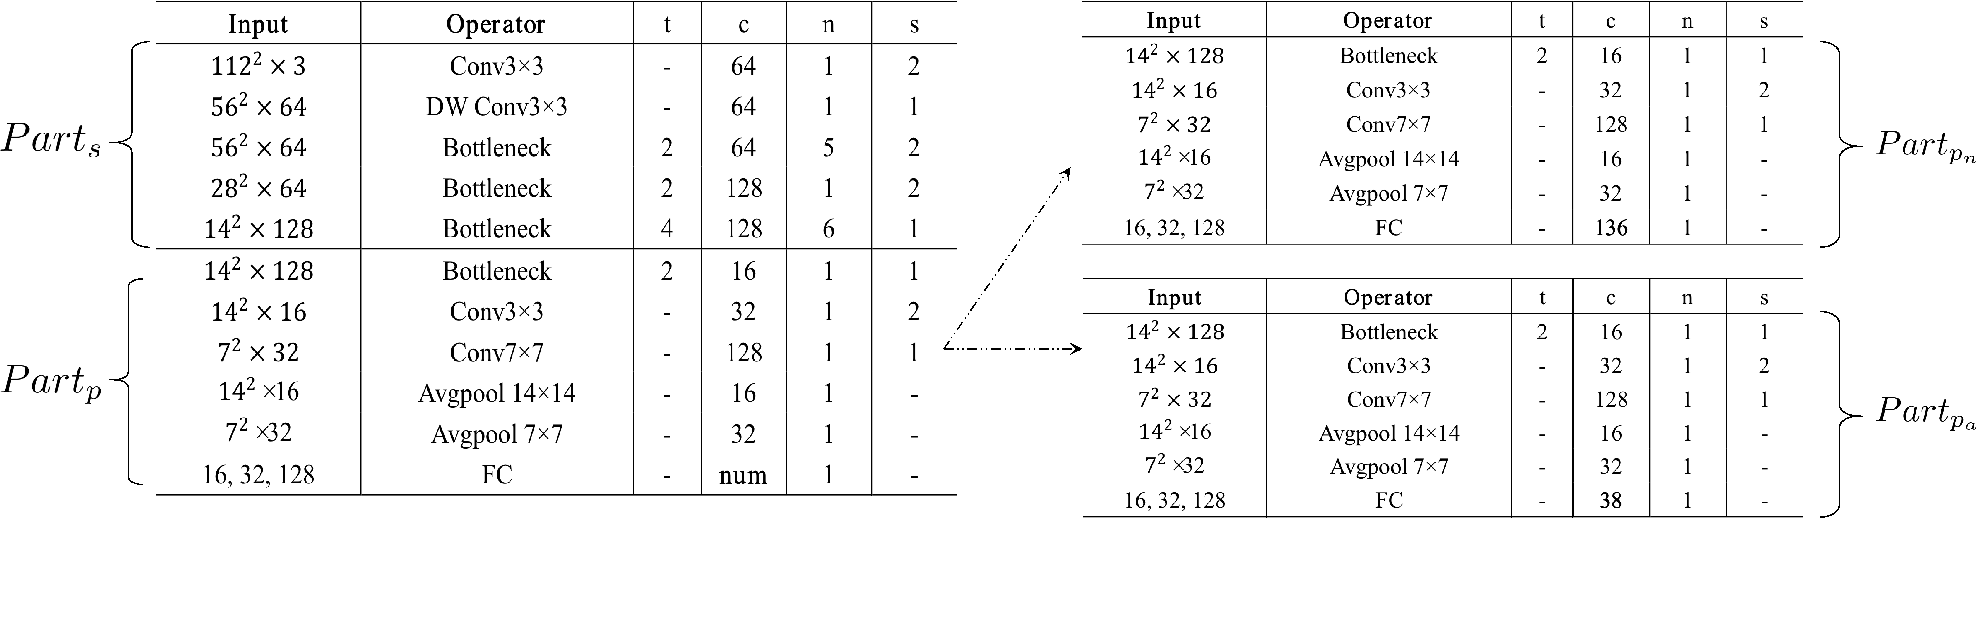
\includegraphics[width=\linewidth]{resize_configuration_direct.eps}
   \caption{The structure of the direct-regression network with network deformation.}
   \label{fig:OCNMP}
 \end{figure*}


During the training process,  ATF utilizes random iterations from different datasets to enable the $Part_s$ to share the parameters, 
which implements the hard parameter sharing.
We also exploit decreasing proportion to enhance the ability to fit the target task.
In the first situation, our evaluation is on only target benchmark even though training on all datasets $\{D_i\}_{i=1}^n$.
Thus, we take validation data or test data of the target dataset as test, which is the same as common training.
For the first scenario, the goal of ATF is to minimize the normalized mean error between the ground-truth points and predictions as below:

% Our method leverages alternating iterations in training to implement hard parameter sharing, which uses multiple datasets for robust sharing part.
% Coupled with alternating training, we also use decreasing proportion to improve the ability of fiting the target task.
% Although all these datasets $\{D_i\}_{i=1}^n$ are used for training, not every dataset is needed for testing.
% As same as normal training, we use the validation set or test set of main dataset $D_n$ as the test.
% Therefore, our goal (not training loss) of the framework is the same as normal to minimize the error between the prediction and the ground truth from testset as below:
\begin{equation}
   \label{eq:goal}
   \mathop{\arg\min}_{\{\omega_s,\omega_m\}} \sum_{i=1}^{N_{t}} ||S_{n_i} - \Phi_m(\Phi_s(I_{n_i},\omega_s),\omega_m) ||
\end{equation}

where $N_t$ represents the number of images in testset, 
and $S_{n_i},I_{n_i}$ are corresponding landmarks and input image for $D_n$.
$\Phi_s$ represents the network structure of $Part_s$, 
and $\Phi_m$ is corresponded to the network structure of $Part_n$ (suppose $Part_n$ is corresponded to the target detector $M_n$).
$\Phi_m(\Phi_s(I_{n_i},\omega_s),\omega_m)$ represents the feature vector of one sample $I_{n_i} \in D_n$.
We use $\omega_s$ to represent the parameters of $Part_s$,
and $\omega_m$ is the parameters of $Part_m$.
When only inference in the target detector, we may prune other private parts $\{Part_{p_i}\}_{i=1}^{n-1}$ for minimizing latency.

During the training process, suppose $I_{ij}$ denotes the $j$-th iteration whose batch data is from $D_i$.
% And one batch consists of equal numbers of images and landmark from one training dataset.
Alternating training leverages sufficient variations of facial features from multiple datasets.
Suppose $r_0,r_1,\dots,r_n$ is the proportion in one epoch corresponded to relative dataset.
We adjust the ratios decreasing to enhance the fitting ability of the target branch $Part_{p_i}$.
The ratios vary as follows: 

\begin{equation}
\label{equation:ratiosDecline}
   (r_0, r_1, \dots, r_n) = (\alpha,\beta,\dots,1)^{ce} \times (r_0, r_1, \dots, r_n)
\end{equation}

Where $\alpha$ and $\beta$ are less than $1$ and represent the coefficient of descent, considered by dataset capacity and markup variance.
$ce$ is the number of the current epoch, and ratios decline in every epoch. 

The following pseudo-code shows the training process of the whole method.


\begin{algorithm}[tbh]
\caption{The training pipeline of our proposed framework}
\label{alg:ATF}
\begin{algorithmic}[1]
\Require
A network with sharing part $\Phi_s$ and multiple branches $\Phi_m , \Phi_a$,  different kinds of iterations $I_m,I_a$ corresponded to datasets.
\State{Set initial ratios of iterations in $Random$}
\For{epoch = 1,2,$\dots,End$}
   \While{current iteration not End}
      \State{$I = next(Random(I_m,I_a))$}
      \State{Forward sharing part $F_s = \Phi_s(I,\omega_s)$}
      \State{Forward branches $P_m=\Phi_s(F_s,\omega_m), P_a=\Phi_a(F_s,\omega_a)$}
      \State{Optimize $\omega_s, \omega_a, \omega_m$ by $\mathcal{L}_{MB}$ defined in Eq.\ref{eq:MBL}} 
   \EndWhile
   \State{Test goal for validation according to Eq.\ref{eq:goal} }
   \State{Change random ratios of iterations via Eq.\ref{equation:ratiosDecline}}

\EndFor
\end{algorithmic}

\end{algorithm}


In the training process, suppose we have five random iterations ($a_1,b_1,a_2,c_1,b_2$) are from different datasets ($A,B,C$) where $a_1,a_2$ are corresponded to $A$.
When training on $b_1$, the model leverages the checkpoint from training on $a_1$ as pretraining and serves the pretraining checkpoint for the next iteration $a_2$.
ATDP makes the networks shared their parameters via randomly finetuning on different datasets.

\subsection{Mixed Branch Loss}
\label{subsec:MBL}

% Although ATDP makes the sharing part shared according hard parameter sharing, the regression parts are still independently learning own inductive bias.
However, the regression parts are still independently learning their own inductive bias. 
To address the issue, we are inspired by the following phenomenon.

Despite the gap that exists in the markup protocol, annotation variance, and capacity among the labels of landmark datasets, 
some keypoints still are well labeled with the same geometric meaning across datasets, \emph{i.e.} eye corners, nose tip.
Although they are a little different in the annotation schemes, their distributions of location are similar.
As shown in figure \ref{fig:Landmark_distribution}, similar landmarks can usually be found among the datasets though markup protocols are different.
There are always 8 to 16 similar landmarks annotated on a pair of datasets (300W\cite{300W}, WFLW\cite{LABWFLW}, COFW\cite{COFW}, AFLW\cite{AFLW}).
These keypoint pairs provide a chance to transfer information from one dataset to the other detector.

Our proposed loss function ($\mathcal{L}_{MB}$) takes advantage of the above information of these similar landmarks to constrain irrelevant branches, especially private parts $\{Part_p\}_{i=1}^{n}$. 
In addition to the native loss, $\mathcal{L}_{MB}$ also constrain the difference between a pair of similar landmarks predicted by different branches.
It can be formulated as follows:

\begin{equation}
   \label{eq:MBL}
   \mathcal{L}_{MB} =
   \begin{cases}
      \mathcal{L}_{m} + \alpha \times \mathcal{L}_{ps} & \text{$ I_i \in D_{m}$} \\
      \beta \times \mathcal{L}_{a} + \gamma \times \mathcal{L}_{ps} & \text{otherwise}
   \end{cases}
\end{equation}


where $I_i$ is the random iteration from a dataset in the current stage, and the proportionality in an epoch corresponds to equation \ref{equation:ratiosDecline}.
We use $\mathcal{L}_m$  to denote the distance between the ground-truth coordinate $S_n$ from target dataset $D_n$ and prediction from target branch  $Part_s + Part_{p_n}$,
$\mathcal{L}_a$ is denoted as the error between the ground-truth coordinate $\{S_i\}_{i=1}^{n-1}$ from auxiliary datasets $\{D_i\}_{i=1}^{n-1}$ and prediction from auxiliary branches $Part_s + \{Part_i\}_{i=1}^{n-1}$, 
and $\mathcal{L}_{ps}$ represents the error between the similar landmarks which are predicted by corresponding $Part_p$.
The weight hyperparameters $\alpha$, $\beta$, $\gamma$ depend on database capacity, markup protocol, and annotation scheme.

Following the previous works\cite{feng2018wing,HRNET,guo2019pfld}, the optimization methods in heatmap-based and direct coordinate are different.
The heatmap-based method needs to calculate the error of each heatmap.
% In the heatmap-based method, we need to calculate the error of each pixel in each heatmap.
Taking the most common second normal form in heatmap\cite{kowalski2017deep,HRNET}, the detailed representation of $\mathcal{L}_{MB}$ in HRNet with multiple parts (HRNETMP) is as follows:


\begin{equation}
\begin{cases}
\begin{split}
&\mathcal{L}_{m}^{H} = \frac{1}{N_{I}^{m} \cdot N_{L}^{m}}  \sum_{i}^{N_{I}^{m}}\sum_{j}^{N_L^m}\sum_k^H\sum_l^W || P_{(i,j,k,l)}^m - V_{(i,j,k,l)}^{gt_m} ||_2^2  \\ 
&\mathcal{L}_{a}^{H} = \frac{1}{N_{I}^{a} \cdot N_{L}^{a}} \sum_{i}^{N_{I}^{a}}\sum_{j}^{N_L^a}\sum_k^H\sum_l^W || P_{(i,j,k,l)}^a - V_{(i,j,k,l)}^{gt_a} ||_2^2  \\ 
&\mathcal{L}_{ps}^{H} =\frac{1}{N_{I}^{m/a} \cdot N_{L}^{s}} \sum_{i}^{N_{I}^{m/a}}\sum_{j}^{N_L^s}\sum_k^H\sum_l^W || P_{(i,j,k,l)}^{sm} - P_{(i,j,k,l)}^{sa} ||_2^2
\end{split}
\end{cases}
\end{equation}

where $N_I^m$ and $N_I^a$ represent the capacities of $D_n$ and $\{D_i\}_{i=1}^{n-1}$,
$N_L^m$, $N_L^a$ and $N_L^s$ denote the number of landmarks in $S_n$ , $\{S_i\}_{i=1}^{n-1}$ and their similar pairs.
$H,W$ are the height and width of heatmap image, $P^m,P^a$ represent the landmark value predicted by target branch and auxiliary branch.
$V^{gt_i}$ is the ground truth value in $S_i$.
$N_{I}^{m/a}$ is $N_I^m$ or $N_I^a$, which is depend on the current iteration.
$P^{sm} \text{ and } P^{sa}$ represent the value in the set of similar pairs, $P^{sm} \in P^{m} \text{ and } P^{sa} \in P^{a} $. 

For direct coordinate regression, the calculation of error is the distance between relative landmarks,
And Feng \emph{et al.}  \cite{feng2018wing} proposes 1st NF are better suitable for direct regression than 2nd NF, the formula of $\mathcal{L}_{MB}$ in OCN with multiple parts (OCNMP) is as follows:

\begin{equation}
\begin{cases}
\begin{split}
&\mathcal{L}_{m}^{D} = \frac{1}{N_{I}^{m} \cdot N_{L}^{m}} \sum_{i}^{N_{I}^{m}}\sum_{j}^{N_L^m} || (P_{(i,j)}^{m_x},P_{(i,j)}^{m_y}) - (V_{(i,j)}^{m_x},V_{(i,j)}^{m_y})||_{1} \\ 
&\mathcal{L}_{a}^{D} =\frac{1}{N_{I}^{a} \cdot N_{L}^{a}} \sum_{i}^{N_{I}^{a}}\sum_{j}^{N_L^a} || (P_{(i,j)}^{a_x},P_{(i,j)}^{a_y}) - (V_{(i,j)}^{a_x},V_{(i,j)}^{a_y})||_{1} \\
&\mathcal{L}_{ps}^{D} = \frac{1}{N_{I}^{m/a} \cdot N_{L}^{s}} \sum_{i}^{N_{I}^{m/a}}\sum_{j}^{N_L^s} || (P_{(i,j)}^{sm_x},P_{(i,j)}^{sm_y} ) - (P_{(i,j)}^{sa_x},P_{(i,j)}^{sa_y})||_{1}
\end{split}
\end{cases}
\end{equation}

where $N_I^m, N_I^a, N_L^m, N_L^a, N_{I}^{m/a} \text{ and } N_L^s$ are the same definition as before.
$P^{sm} \text{ and } p^{sa}$ are similar with the above definition, which are changed from a pixel value to a couple coordinate.
$P_{(i,j)}^{m_x},P_{(i,j)}^{m_y}$ are the x- and y-coordinate of $j$-th in $i$-th image, which is predicted by main branch $P^m$.
$P_{(i,j)}^{a_x},P_{(i,j)}^{a_y}$ are the x- and y-coordinate of $j$-th in $i$-th image, which is predicted by auxiliary branch $P^a$.
$(V_{(i,j)}^{m_x},V_{(i,j)}^{m_y})$ is the ground truth coordinate of $j$-th in $i$-th image of $D_n$.
$(V_{(i,j)}^{a_x},V_{(i,j)}^{a_y})$ is the ground truth coordinate of $j$-th in $i$-th image of the auxiliary dataset.

Although we conduct experiments with 1st NF and 2nd NF loss functions, it should be noted that our method is also applicable to other common loss functions as the original one.


\subsection{Extending to Common Scenarios}
\label{extend common}
In practical applications, it will cost more computations and GPU memory if we use ATF directly.
Thus, we have done some optimizations for ATF to extend to three situations: when the target detector is enough, when a joint detector including all source detectors is needed, when a new novel detector is coming.

% As detailed discuss in the above subsections, we mainly consider the first case.
For the situation where only the target detector is needed, auxiliary detectors are useless and consume resources in the test stage.
We keep the sharing part $Part_s$ and the target branch $Part_{p_n}$ unchanged, pruning all auxiliary branches $Part_{p_1},Part_{p_2},\dots,Part_{p_{n-1}}$, so that the optimized networks structure is consistent with the original model. 

Due to the different annotation schemes, there always exists the meet that a joint detector including more than one even all detectors aims to get as many points as possible. 
Our framework uses only one shared backbone, and multiple regression branches, which greatly reduces the amount of calculation and GPU memory compared with other methods \cite{smith2014collaborative,zhu2014transferring}.
Compared with the original detector, ATF adds a little computing resource and realizes multiple detectors.
However, the immediate use of ATF will leave a gap in its peak performance on the auxiliary datasets. 
To bridge this gap, it is recommended to finetune the network on its data independently.
Moreover, limited by the resources and training time, we freeze the parameters of the sharing part and only finetune the parameters of the private branches with each dataset.
The results are shown in the subsection.\ref{extend experiments}, which demonstrate that our backbone is robust enough for the rarely or unseen variations.


It is common to construct an accurate detector on a new facial landmark dataset, 
and the novel landmark is with different schemes.
Intuitively, restarting training from zero to be finished is time-consuming.
We propose a simple and fast method to obtain an accurate enough detector via our framework.
Add another private part to the original ATF, and this branch should correspond to the new labels.
Freeze the parameters of the sharing backbone, and finetune the new regression branch.
Comparing with re-training, ATF takes less than 1/10 of the time and obtains comparable or even higher accuracy.
Although we only finetune on regressional parts, it should be noted that finetuning the entire network will achieve higher performance.


\begin{table*}[t]
\begin{center}
\resizebox{0.75\textwidth}{!}{
\begin{tabular}{|c|l|c|c|c|c|c|c|c|c|c|c|}
\hline
Metric & Method & Fullset & \tabincell{c}{Pose} & \tabincell{c}{Exp.} & \tabincell{c}{Ill.} & \tabincell{c}{Mu.} & \tabincell{c}{Occ.} & \tabincell{c}{Blur} \\

\hline\hline
\multirow{12}{*}{$\text{NME}(\downarrow)$} 
   & SDM \cite{xiong2013supervised} & 10.29 & 24.10 & 11.45 & 9.32 & 9.38 & 13.03 & 11.28 \\
~& CFSS \cite{zhu2015face} & 9.07 & 21.36 & 10.09 & 8.30 & 8.74 & 11.76 & 9.96 \\
~& DVLN \cite{wu2017leveraging} & 6.08 & 11.54 & 6.27 & 5.73 & 5.98 & 7.33 & 6.88 \\
~& LAB \cite{LABWFLW}& 5.27 & 10.24 & 5.51 & 5.23 & 5.15 & 6.79 & 6.32 \\
~& PDB \cite{feng2018wing} & 5.11 & 8.75 & 5.36 & 4.93 & 5.41 & 6.37 & 5.81 \\
~& DCFE \cite{valle2018deeply} & 4.69 & 8.63 & 6.27 & 5.73 & 5.98 & 7.33 & 6.88 \\
~& DeCaFA \cite{dapogny2019decafa} & 4.62 & 8.11 & 4.65 & 4.41 & 4.63 & 5.74 & 5.38 \\
~& AS w. SAN \cite{qian2019aggregation} & {\bf 4.39 } & 8.42 & 4.68 & {\bf 4.24} & 4.37 & 5.60 & {\bf 4.86} \\

\cline{2-9}\cline{2-9}
~& OCN & 4.93 & 8.94 & 5.05 & 5.13 & 5.00 & 5.95 & 5.62 \\
~& OCNMP & 4.60 & 8.05 & 4.69 & 4.66 & 4.60 & 5.54 & 5.20 \\
~& HRNET \cite{HRNET}  & 4.60 & 7.94 & 4.85 & 4.55 & 4.29 & 5.44 & 5.42 \\
~& HRNETMP & 4.50 &  {\bf 7.54} & {\bf 4.65} & 4.45 & {\bf 4.20} & {\bf 5.30} &  5.19 \\
\hline

\multirow{12}{*}{$\text{FR}_{10}(\downarrow)$} 
   & CFSS \cite{zhu2015face}             & 20.56 & 66.26 & 23.25 & 17.34 & 21.84 & 32.88 & 23.67 \\
~ & DVLN \cite{wu2017leveraging}        & 10.84 & 46.93 & 11.15 & 7.31  & 11.65 & 16.30 & 13.71 \\
~ & LAB \cite{LABWFLW}                  & 7.56  & 28.83 & 6.37  & 6.73  & 7.77  & 13.72 & 10.74 \\
~ & Wing \cite{feng2018wing}            & 6.00  & 22.70 & 4.78  & 4.30  & 7.77  & 12.50 & 7.76  \\
~ & DeCaFA \cite{dapogny2019decafa}     & 4.84  & 21.40 & 3.73  & 3.22  & 6.15  & 9.26  & 6.61  \\
~ & AS w. SAN \cite{qian2019aggregation}& 4.08  & 18.10 & 4.46  & 2.72  & 4.37  & 7.74  & 4.40  \\
% ~ & AWing \cite{wang2019adaptive}       & \textbf{2.84}  & \textbf{13.50} & 2.23  & 2.58  & 2.91  & 5.98  & 3.75  \\
% ~ & LUVLI \cite{kumar2020luvli}         & 3.12  & -  & - & -  & -  & -  & -  \\
\cline{2-9}\cline{2-9}
~& OCN & 5.92 & 27.00 & 5.10 & 5.16 & 6.80 & 10.46 & 5.69 \\
~& OCNMP & 4.52 & 20.15 & 3.18 & 3.58 & 5.83 & 8.42 & 4.53 \\
~& HRNET &  3.12 & 16.26 & 2.55 & 2.72 & 1.94 & 5.71 &  4.53 \\
~& HRNETMP & {\bf 2.52} & {\bf 13.19} & {\bf 2.23} & {\bf 2.44} & {\bf 0.49} & {\bf 5.03} &  {\bf 3.88} \\
\hline

\multirow{12}{*}{$\text{AUC}_{10}(\uparrow)$} 
   & CFSS \cite{zhu2015face}             & 0.366 & 0.063 & 0.316 & 0.385 & 0.369 & 0.269 & 0.303 \\
~ & DVLN \cite{wu2017leveraging}        & 0.456 & 0.147 & 0.389 & 0.474 & 0.449 & 0.379 & 0.397 \\
~ & LAB \cite{LABWFLW}                  & 0.532 & 0.235 & 0.495 & 0.543 & 0.539 & 0.449 & 0.463 \\
~ & Wing \cite{feng2018wing}            & 0.554 & 0.310 & 0.496 & 0.541 & 0.558 & 0.489 & 0.492 \\
~ & DeCaFA \cite{dapogny2019decafa}     & 0.563 & 0.292 & 0.546 & 0.579 & 0.575 & 0.485 & 0.494  \\
~ & AS w. SAN \cite{qian2019aggregation}& {\bf 0.591} & {\bf 0.311} & {\bf 0.549} & {\bf 0.609} & {\bf 0.581} & {\bf 0.516} & {\bf 0.551} \\
% ~ & AWing \cite{wang2019adaptive}       & 0.572 & 0.312 & 0.515 & 0.578 & 0.572 & 0.502 & 0.512 \\
% ~ & LUVLI \cite{kumar2020luvli}         & 0.577  & -  & - & - & -  & - & - \\

\cline{2-9}\cline{2-9}
~& OCN & 0.5388 & 0.2407 & 0.5121 & 0.5544 & 0.5242 & 0.4604 & 0.4885 \\
~& OCNMP & 0.5615 & 0.2897 & 0.5339 & 0.5753 & 0.5449 & 0.4853 & 0.5156 \\
~& HRNET & 0.5536 & 0.2867& 0.5360 & 0.5623 & 0.5770 & 0.4965 &  0.4969 \\
~& HRNETMP & 0.5604 & 0.3010 & 0.5460 & 0.5663 & {\bf 0.5806} & 0.4874 &  0.4893 \\
\hline


\end{tabular}
}
\end{center}
\caption{Comparisons in inter-ocular normalized mean error (NME), area under curve (AUC) and failure rate (FR) on the WFLW (fullset and all subsets). Note HRNet's paper does not offer the information about AUC and FR, and we take its checkpoint from the offical code.}
\label{tab1_WFLW}
\end{table*}


\begin{table*}[t]
\begin{center}
\resizebox{0.5\textwidth}{!}{

\begin{tabular}{|l|c|c|c|c|c|}
\hline
Method  & \tabincell{c}{300W \\ Full} & \tabincell{c}{300W \\Com.} & \tabincell{c}{300W \\ Cha. } & \tabincell{c}{COFW \\Full} & \tabincell{c}{AFLW \\ Full}   \\
\hline\hline

RAR \cite{xiao2016robust}  & - & - & - & 6.03 & - \\
RCN \cite{honari2016recombinator}  & 5.41 & 4.67 & 8.44 & - & 5.6  \\
DAN \cite{kowalski2017deep}  & 3.59 & 3.19 & 5.24 & - & - \\
DAC-CSR \cite{feng2017dynamic} & - & - & - & 6.03 & 2.27  \\
SAN \cite{dong2018style} &  3.98 & 3.34 & 6.60 & - & 1.91  \\
RCN+ \cite{honari2018improving} &  4.90 & 4.20 & 7.78 & - & 1.61  \\
PDB \cite{feng2018wing} &  3.60 & 3.01 & 6.01 & - & {\bf 1.47}  \\
LAB \cite{LABWFLW} &  3.49 & 2.98 & 5.19 & 5.58 & 1.85  \\
DCFE \cite{valle2018deeply}&  3.24 & 2.76 & 5.22 & - & 2.17  \\
$\text{TS}^3$ \cite{dong2019teacher}  & 3.78 & 3.17 & 6.41 & - & 1.99 \\
LaplaceKL \cite{robinson2019laplace}  & 4.01 & 3.28 & 7.01 & - & 1.97  \\
ODN \cite{zhu2019robust}  & 4.17 & 3.56 & 6.67 & 5.3 & 1.63  \\
AS w. SAN \cite{qian2019aggregation}  & 3.86 & 3.21 & 6.49 & - & -  \\
HG-HSLE \cite{zou2019learning}  &  3.28 & 2.85 & 5.03 & - & -  \\
\hline\hline
OCN  & 3.87 & 3.36 & 5.84 & 4.18 & 2.00  \\
OCNMP & 3.55 & 3.12 & 5.32 & 3.91 & 1.91  \\
HRNET \cite{HRNET}  & 3.32 & 2.87 & 5.15 & 3.45 & 1.57 \\
HRNETMP  & {\bf 3.17} & {\bf 2.75} & {\bf 4.89} & {\bf 3.32} & 1.55 \\

\hline
\end{tabular}
  }
\end{center}
\caption{Comparison in inter-ocular normalized mean error (NME) on the 300W (common subset, Challenging subset, and fullset), COFW  and AFLW.}
\label{tab1_300W}
\end{table*}

\section{Experiments}
\label{sec:experiments}
\subsection{Experimental Settings}
{\bf Datasets }  We conduct extensive experiments on widely used benchmarks \cite{300W,AFLW,LABWFLW,COFW}. 
These datasets are challenges because facial images focus on variations in makeup, extreme pose, and wide occlusion.

\emph{300W}\cite{300W} data set offers 68 keypoints for each 2D face, which are collected from AFW\cite{zhu2012face}, HELEN\cite{le2012interactive}, LFPW\cite{belhumeur2013localizing},  XM2VTS\cite{messer1999xm2vtsdb}, and IBUG. 
According to the protocol used in \cite{zhu2012face}, all 3148 training images are from the training set of LFPW and HELEN and the full set of AFW. 
The 689 test images come from the test collection of LFPW and HELEN, as well as the full set of IBUG. 
The test images are further divided into three subsets: 554 samples from LFPW and HELEN as the common subset, the 135-image IBUG as the challenging subset, and their union as the full set.

\emph{WFLW}\cite{LABWFLW} dataset is the most challenging benchmark, which contains 7,500 face images for training and 2,500 images for the test.
And WFLW is the newest benchmark based on WIDER Face\cite{yang2016wider} with 98 manually annotated keypoints. 
The faces images introduce many types of variations concerning large pose, expression, occlusion, etc. 
The test set is further divided into six subsets for comprehensive evaluation: pose (326 images), expression (314 images), illumination (698 images), make-up (206 images), occlusion (736 images), and blur (773 images).


\emph{COFW}\cite{COFW} dataset contains 1345 images for training and 507 images for the test, and each face image has been annotated with 29 landmarks.
In this dataset, the face data focus on large variations and occlusions. 

\emph{AFLW}\cite{AFLW} dataset is annotated with 19 landmarks, which contains 24386 wild faces with large head pose up to $120^{\circ}$ for yaw and $90^{\circ}$ for pitch and roll. 
According to the previous protocol \cite{zhu2015face,zhu2016unconstrained}, the AFLW-full uses 20000 images for training and 4386 images for the test.
% The subset AFLW-Frontal is to evaluated frontal images, which consists of 1314 images from the testset.

% is widely used for benchmarking facial landmark localization with 19 landmarks, which contains 24386 in-the-wild
% faces with large head pose up to $120^{\circ}$ for yaw and $90^{\circ}$ for pitch and roll. 
% Following the widely-adopted protocol\cite{zhu2015face,zhu2016unconstrained}, the AFLW-full dataset has 20000 images for training and 4386 for testing. 
% And the AFLW-Frontal contains 1314 images selected from 4386 testing images for evaluation frontal images.

{\bf Baseline networks} We take OCN and HRNet as baselines for direct coordinates regression and heatmap-based regression.
OCN exploits the bottleneck \cite{sandler2018mobilenetv2} like \cite{guo2019pfld} to construct the network.
It uses the  $112 \times 112 \times 3$ as the input resolution and coupled with $L1$ loss following previous practice \cite{feng2018wing,guo2019pfld}.
HRNET uses the backbone of HR-18\cite{HRNET} and take the $256 \times 256 \times 3 $ as input shape, which combine $L2$ loss for optimization.
We transform the baseline networks to get new networks with multiple private parts, noted as OCNMP and HRNETMP.
For simplicity, we add the first letter of dataset name behind the network name, denoted as multiple $Part_p$.
For example, $OCNMP_{W3}$ means OCNMP has two private parts, one corresponding to WFLW\cite{LABWFLW} and the other corresponding to 300W\cite{300W}.

% For HRNETMP, we leave the head layers for private part.
% And for OCNMP, except fully-connect layers, we add a few convolutional layers and average pooling layers for private parts.


{\bf Evaluation Metrics} Following most previous works\cite{HRNET,kumar2018disentangling,LABWFLW,dong2018style}, 
we take normalized mean error (NME), area under the curve (AUC) and failure rate (FR) as metrics to comprehensive verify our method.

\emph{Normalized Mean Error (NME)} is the most authoritative and used for face alignment.
We take the outer-eye-corner distance as the normalizing factor for WFLW\cite{LABWFLW}, COFW\cite{COFW}, and 300W\cite{300W}, 
and the face size as the normalizing factor for AFLW because of various profile faces\cite{AFLW}. 
NME is defined as:

\begin{equation}
   NME(\%) = \frac{1}{N} \sum_{k = 1}^{N} \frac{||P_k-\hat{P_k}||_2}{d} \times  100
\end{equation}

where the normalized factor $d$ represents the distance between the outer corners of the left and right eyes. 
$P_k \text{ and } \hat{P_k}$ represent the ground-truth coordinate and prediction of the $k$-th keypoint.
For simplicity, we magnify 100 times to omit the \% symbol. 
Lower NME is for better performance.

\emph{Area Under the Curve (AUC)} is calculated based on the cumulative error distribution (CED) curve.
The AUC for a test set is computed as the area under the curve, up to the cut-off NME value.
Higher AUC represents a better detector.
To compare with previous methods, the AUC and FR are used on WFLW fullset and all subsets.

\emph{Failure Rate (FR)} is another metric to evaluate localization quality, which refers to the percentage of images in the testset when NME is larger than a prefixed threshold.
And we also omit the \% symbol to simplify variables.
The Lower FR is corresponding to better performance.


{\bf Implementation Details} 
When conduct experiments on OCN and OCNMP, we crop and resize all image data of the target detector to $112\times 112 \times 3 $ resolution via the facial boxes from retina-face detector\cite{deng2020retinaface}.
We set the initial learning rate to 1e-3 with Adam optimization.
The data augmentation contains random crop(0.2), horizontal flipped(0.5), and rotation($\pm$30).
The learning rate will decrease by 0.1 times if the loss of validation stops decrease in 10 epochs.
For a fair comparison, the experiment settings on HRNETMP are the same as HRNet\cite{HRNET}.
In the experiments concerning alternating training, we also adjust iteration ratios for one epoch.
We set the initial proportion to 2:1 or 3:1 and set ratios from 0.8 to 0.95, depending on the dataset capacity and markup schemes.
And loss weights $\alpha,\beta,\gamma$ are decided by the annotation protocol and dataset capacity, which also exist a little distinguish in each pair.
Especially, when leveraging AFLW as auxiliary and WFLW as main, we set $\alpha \text{equals} 0.2, \beta \text{equals} 0.8 , \gamma \text{equals} 0.1$.


% For experiments on heatmap-based model (HRNET,HRNETMP), 
% all training images data of the target dataset are cropped and resized to $256\times 256 $ according to provided bounding boxes.
% And we use Adam technique for optimization with an initial learning rate of 1e-4.
% To be consistent with base model, the learning rate decrease by 0.1 times at 30 and 50 epochs, and the training ended at 60 epochs.
% We only use three data augmentation for training data: random cropping, horizontal flipping, and rotation.
% Note testing images are cropped and resized using provided bounding boxes \emph{without any spatial transformation} for fair comparison with other methods.

% And for experiments on direct coordinate model (OCN, OCNMP),
% all training images data of the $D_m$ are cropped and resized to $112\times 112 $ according to the boxes predicted by retina face detector.
% And we also use Adam with an initial learning rate of 1e-3.
% The learning rate will decrease by 0.1 times when the loss of validation do not decrease in 10 epoch.
% The ways of data augmentation are similar as above except pixel changes.

% In alternating training, we also need set iteration proportions in one epoch. 
% We usually start at 2:1 or 3:1, and set $ratios$ about 0.8 to 0.95.
% The loss hyperparameters $\alpha,\beta,\gamma$ depend on the difference of the annotation protocol and capacity.
% For example, using AFLW to assist WFLW,  we set $\alpha = 0.2, \beta=0.8 , \gamma=0.1$ 
% And the pair of auxiliary dataset and main dataset is different, the hyperparameters also exist a few distinguish.  


\subsection{Comparison with State-of-the-art Methods}
We firstly conduct experiments with OCN on each benchmark to obtain the baseline result.
Next, we use the union database of multiple datasets to train OCNMP and HRNETMP, which take OCN and HRNET\cite{HRNET}'s results as baselines.
To verify the effectiveness, we further compare OCNMP, HRNETMP with the state-of-the-art works on each benchmark.
Note OCN again is a slight network with 1.228M parameter and 279.96M FLOPs, and the model size of HRNET is 9.663M parameters and 4.734G FLOPs.
As shown in Tab.\ref{tab1_WFLW}, the result about WFLW fullset and subsets are impressive.
Note that the FR and AUC of HRNet are evaluated from the official checkpoint.
The Tab. \ref{tab1_300W} shows the normalized mean error on 300W, AFLW, and COFW, including their fullsets and subsets.
At all fullset and subsets, ATF improves the performance of the detector in each network.
% The results on 300W, AFLW and COFW are showed in Table \ref{tab1_300W}.
% And Table \ref{tab1_WFLW} shows our performance on the testset and subsets of WFLW.

Compared with HRNet, HRNETMP leveraging ATF has obtained obvious improvement in various benchmarks.
And on experiments on 300W, COFW, and AFLW, HRNETMP outperforms other SOTA methods by a lot. 
Especially, the NME of ATF reaches 3.17, 2.75, and 4.89 for fullset and subsets of 300W\cite{300W}, 3.32 for COFW fullset, 1.55 for AFLW.
Compared with the HRNet baseline, it achieves a huge enhancement on 300W, $4.5\%$, $4.1\%$, and $5.04\%$ relative ascension.
Moreover, we extend three metrics on WFLW, HRNETMP always performs best at FR and NME, particularly 2.52 for failure rate.
The experiments on WFLW fullset and all subsets demonstrate that our method is useful for all benchmarks.
This phenomenon is noticeable on the challenge dataset.
Especially, the large-pose subset includes data with relatively large Euler angles and severe self-occlusion.
The ascension on this subset reaches 5.41\%, which is higher than other improvements.
And experiments on 300W, the enhancement of the challenge subset ($5.04\%$) is more significant than the common subset ($4.1\%$).
The above phenomenon demonstrates that our framework makes it possible to learn the data variations which is rarely or unseen in the original dataset.
% And it also obtains the improvement comparing with baseline on AFLW and COFW benchmarks.


% On experiments with HRNETMP, our method significantly outperforms best among state-of-the-art methods by a large margin.
% And HRNETMP performs better than baseline HRNET. 
% Note it achieve $3.17, 2.75, 4.89$ NME for fullset, common subset and challenging subset on 300W\cite{300W}.
% It equals $4.5\%$, $4.1\%$ and $5.04\%$ relative performance improvement over the baseline method.
% On COFW and AFLW, our approach in heatmap-based HRNETMP also has minor improvement than before HRNET.
% As shown in Tab.\ref{tab1_WFLW}, we test performance of our model on the subsets of WFLW.
% And the result shows our method are beneficial to all subsets.
% Especially, the performance on the WFLW benchmark of the large-pose subset has higher relative improvement 5.41\% than other subsets.
% And the performance on the 300W benchmark of the challenge subset performs higher ascension 5.04\% than other subsets.
% We find that HRNET with training by ATF can decrease the error in more difficult testset obviously.

On the experiments with the slight network, OCNMP obtains bigger relative improvement than HRNETMP.
Leveraging ATF again makes obvious improvement on each benchmark than original training. 
As shown in Tab.\ref{fig:OCNMP}, OCNMP reaches 4.60 on the WFLW fullset and 3.55 on 300W, which is comparable to the SOTA result.
Thus, OCNMP provides a great trade-off between accuracy and computation.
Comparing with the OCN baseline, OCNMP achieves $4.5\%$ relative ascension for AFLW, $8.24\%$ for 300W, $6.81\%$ for WFLW, and COFW $6.55\%$.
Moreover, ATF works well on not only the fullset but also all subsets, $7.14\%$ for 300W Common, $8.90\%$ for 300W Challenge, $7.12\%$ for WFLW expression etc.
In particular, the enhancements of the challenge subsets are higher, $8.9\%$ for cha subset and $9.96\%$ for pose subset.
Again, ATF achieves obvious enhancement comparing with original training, and the performance outperforms SOTA by a large margin.

We also have visualized some cases on WFLW as shown in Fig.\ref{fig:visualize}. The pictures from left to right are  raw image (input image), HRNet\cite{HRNET} output, ATF output (ours) and ground-truth.
% On the experiments with slight network OCNMP, ATF still achieves obvious ascension than before OCN among every benchmarks.
% The way that ATF training the multiple datasets simultaneously makes it possible for learning the unique ability which is in unseen domain.
% OCNMP gets $4.5\%$, $8.24\%$, $6.81\%$ and $6.55\%$ relative performance improvement over OCN on AFLW, 300W, WFLW and COFW.
% with ATF, OCN gets higher relative performance improvement than HRNET in all benchmarks.
% Also in the direct coordinate regression method, we find that the relative performance improvement on difficult subset is obvious higher than other subsets.
% In particular, the improvements are 8.9\% in 300W cha. 9.96\% in WFLW pose.
% Again, our proposed method achieve significantly improvement and the best performance among state-of-the-art methods.

\begin{table*}[t]
\begin{center}
\resizebox{0.6\textwidth}{!}{
\begin{tabular}{|c|l|c|c|c|c|c|c|c|}
\hline
Network & Method & test & blur & exp. & ill. & pose & mu. & occ. \\
\hline\hline 
\multirow{4}{*}{$\text{OCN}$} 
   & baseline & 4.93& 5.62& 5.05& 5.13& 8.94& 5.00& 5.95 \\
~ & $\text{ATF}_{WC}$ & 4.64& 5.26& 4.66& 4.79& 8.40& 4.79& 5.59 \\
~ & $\text{ATF}_{W3}$ & 4.72& 5.35& 4.86& 4.88& 8.62& 4.86& 5.69 \\
~ & $\text{ATF}_{WA}$ & 4.60& 5.20& 4.69& 4.66& 8.05& 4.60& 5.54 \\
\hline

\multirow{4}{*}{$\text{HRNET}$} 
& baseline & 4.60 & 5.42 & 4.85 & 4.55 & 7.94 & 4.29 & 5.44\\
~ & $\text{ATF}_{WC}$ & 4.54 & 5.30& 4.74& 4.50& 7.56& 4.25& 5.32\\
~ & $\text{ATF}_{W3}$ & 4.52& 5.28& 4.63& 4.44& 7.53& 4.24& 5.29\\
~ & $\text{ATF}_{WA}$ & 4.50& 5.19& 4.65& 4.45& 7.54& 4.20& 5.30\\
\hline
% \hline
% \multirow{4}{*}{$\text{FR}_{10}(\downarrow)$} 
% & baselines & - & - & - & - & - & - & - \\
% ~ & $\text{ATF}_{WC}$ & - & - & - & - & - & - & - \\
% ~ & $\text{ATF}_{W3}$ & - & - & - & - & - & - & - \\
% ~ & $\text{ATF}_{WA}$ & - & - & - & - & - & - & - \\
% \hline

% \hline
% \multirow{4}{*}{$\text{AUC}_{10}(\uparrow)$} 
% & baselines & - & - & - & - & - & - & - \\
% ~ & $\text{ATF}_{WC}$ & - & - & - & - & - & - & - \\
% ~ & $\text{ATF}_{W3}$ & - & - & - & - & - & - & - \\
% ~ & $\text{ATF}_{WA}$ & - & - & - & - & - & - & - \\
% \hline

\end{tabular}
}
\end{center}
\caption{Comparison in NME of HRNET with variants and OCN with variants on WFLW benchmark (fullset, and all subsets). $\text{ATF}_{WC}$ denotes COFW assist the target dataset WFLW.}
\label{tab:cross WFLW}
\end{table*}


\begin{table*}[t]
\begin{center}
\resizebox{0.45\textwidth}{!}{
\begin{tabular}{|c|l|c|c|c|c|}
   \hline
   
Network & Method & full & com. & cha. & test \\
   \hline\hline
   \multirow{4}{*}{$\text{OCN}$} 
~ &  baseline & 3.87& 3.39& 5.85& 4.52 \\
~ &   $\text{ATF}_{3C}$ & 3.69& 3.24& 5.53& 4.33 \\
~ &   $\text{ATF}_{3A}$ & 3.56& 3.11& 5.39& 4.19 \\
~ &   $\text{ATF}_{3W}$ & 3.55& 3.12& 5.32& 4.15 \\
   \hline


\multirow{4}{*}{$\text{HRNET}$} 
~ &  baseline & 3.32& 2.87& 5.15& 3.85 \\
~ &   $\text{ATF}_{3C}$ & 3.28& 2.85& 5.08& 3.87 \\
~ &   $\text{ATF}_{3A}$ & 3.24& 2.82& 4.98& 3.77 \\
~ &   $\text{ATF}_{3W}$ & 3.17& 2.75& 4.89& 3.65 \\
   \hline

\end{tabular}
}
\end{center}
\caption{Comparison in NME of networks on 300W benchmark (fullset, common subset and challenge subset). }
\label{tab:cross 300W}
\end{table*}



\subsection{Evaluation ATF on Cross Datasets}
We conduct experiments on the cross dataset to verify the feasibility of the framework.
To demonstrate the robustness of each benchmark, we also experiment on each pair of datasets with OCNMP and HRNETMP.

We firstly experiment on WFLW fullset and all subsets, which the auxiliary dataset is from 300W, COFW and AFLW independently.
The result is showed in Tab.\ref{tab:cross WFLW}, with AFLW assistant, both HRNetMP and OCNMP achieve the best result, $4.60$ for ONCMP and $4.50$ for HRNETMP.
For convenience in network abbreviation, we take C to denote COFW, W for WFLW, A for AFLW, and 3 for 300W. Specifically, $\text{ATF}_{WC}$ denotes COFW assist the target dataset WFLW.
It also obtains significant ascension on all subsets of WFLW, HRNETMP reaches 5.29 for occlusion, OCNMP reaches 4.69 for expression.
Furthermore, makeup and pose subsets are improved, which means the auxiliary dataset contains additional representation focus on pose and makeup.
Although 300W and COFW are with smaller capacities, ATF still improves the performance by leveraging them, which also demonstrates the effectiveness of our framework.

% As shown in tab. \ref{tab:cross WFLW} HRNET with $ATF_{WA}$ gets the highest performance $\mathbf{4.50}$, while OCN with $ATF_{WA}$ gets the highest ascension.
% Although by leveraging small datasets, 300W or COFW, our framework also proves its feasiblility.
% For these sub-benchmarks in WFLW, the performance on pose, makeup is get higher robust than others, which means that ATF learns the extra pose and makeup representations in other datasets.


% To verify the effectiveness of our method on cross datasets,
% we design the experiments on all pairs of datasets with both networks.
% And all results show the effectiveness of our method.

\begin{minipage}{\textwidth}
\begin{minipage}[t]{0.225\textwidth}
\centering
\makeatletter\def\@captype{table}\makeatother
\resizebox{\textwidth}{!}{
\begin{tabular}{|l|c|}        
\hline
HRNET/OCN & test \\
\hline\hline
baselines & 3.45/4.18 \\
$\text{ATF}_{C3}$  & 3.42/3.97 \\
$\text{ATF}_{CA}$  & 3.36/3.95 \\
$\text{ATF}_{CW}$  & 3.32/3.91 \\
\hline
\end{tabular}
}
\caption{Comparison in NME of networks on COFW}
\label{tab:cross COFW}
\end{minipage}
\begin{minipage}[t]{0.225\textwidth}
\centering
\makeatletter\def\@captype{table}\makeatother
\resizebox{\textwidth}{!}{
\begin{tabular}{|l|c|}        
\hline
HRNET/OCN & test \\
\hline\hline
baselines & 1.57/1.99 \\
$\text{ATF}_{A3}$  & 1.56/1.91 \\
$\text{ATF}_{AC}$  & 1.56/1.92 \\
$\text{ATF}_{AW}$  & 1.55/1.91 \\
\hline
\end{tabular}
}
\caption{Comparison in NME of networks on AFLW}
\label{tab:cross AFLW}
\end{minipage}
\end{minipage}


Verified on 300W\cite{300W} benchmark, leveraging WFLW achieves the most significant improvement among datasets in both HRNETMP and OCNMP, 
which is shown in Tab. \ref{tab:cross 300W}.
And the NME reaches to the {\bf 3.17} on fullset, 2.75 on common set, and 4.89 on challenge set, which outperforms SOTA a lot.
Also, utilizing COFW or AFLW to assist 300W independently performs better than baseline, and ATF again demonstrates its robustness for each dataset.
As shown in Tab.\ref{tab:cross COFW}, leveraging WFLW also achieves best among experiments on COFW.
The Tab.\ref{tab:cross AFLW} reveals the result of leveraging auxiliary datasets for AFLW.
The joint performance ($OCNMP_{WA}$, $OCNMP_{C3}$ \emph{et al.}) utilizing multiple datasets outperforms 5\% higher than baseline, even often 8\% higher.
And due to WFLW is the newest public dataset, exploiting WFLW to assist other detectors always obtains the best performance, 
which also shows that the performance of ATF is related to the markup protocol.

% As shown in tab. \ref{tab:cross 300W}, $HRNETMP_{3W}$ performs highest among these variants in heatmap-based method.
% Also,$OCNMP_{3W}$ get the highest performance 3.55 among the variants of OCN.
% As shown in tab.\ref{tab:cross COFW} $HRNETMP_{CW}$ and $OCNMP_{CW}$ also perform the best on COFW benchmark.
% And as shown in tab.\ref{tab:cross AFLW} on AFLW benchmark, ATF with different dataset makes smiliar improvement due to the large amount of AFLW.
% The performance of these variants ($OCNMP_{WA}$, $OCNMP_{C3}$ \emph{et al.}) with training cross datasets is generally 5\% higher than original model, and some even 8\% higher.
% And we find using WFLW to assist another one detector is able to get the target detector with highest accuracy, which it may be related to the latest published dataset(WFLW is newest).

It is demonstrated that ATF is effective in leveraging a union of multiple datasets via the weakly supervised approach.
The above results illustrate that the proposed ATF framework based on either Heatmap-based or direct coordinate regression can exploit sufficient variations in different datasets,
which enhances the variation generalization and produces a highly robust model.
% And it is an interesting phenomenon that using WFLW as auxiliary, we can get the highest improvement among cross datasets.



\begin{table*}[t]
\begin{center}
\resizebox{0.7\textwidth}{!}{
\begin{tabular}{|c|l|c|c|c|c|c|c|c|}
\hline
Metric & Auxiliary & test & blur & exp. & ill. & pose & mu. & occ. \\
\hline\hline 
\multirow{6}{*}{$\text{NME}(\downarrow)$} 
~ & $\text{COFW}_{wod}$ & 4.57 & 5.32 & 4.75 & 4.47 & 7.70& 4.36 & 5.38 \\
~ & $\text{COFW}_{wd}$ & 4.54 & 5.30 & 4.74 & 4.50 & 7.56 & 4.25 & 5.32 \\
~ & $\text{300W}_{wod}$ & 4.56 & 5.29 & 4.72 & 4.52 & 7.67 & 4.22 & 5.41 \\
~ & $\text{300W}_{wd}$ & 4.52 & 5.28 & 4.63 & 4.44 & 7.53& 4.24 & 5.29 \\
~ & $\text{AFLW}_{wod}$ & 4.53& 5.27& 4.74& 4.44& 7.65& 4.31& 5.32 \\
~ & $\text{AFLW}_{wd}$ & 4.50& 5.19& 4.65& 4.45 & 7.54 & 4.20& 5.30 \\
\hline

\hline
\multirow{6}{*}{$\text{FR}_{10}(\downarrow)$} 
~ & $\text{COFW}_{wod}$ & 2.84 & 4.01 & 2.23 & 2.44 & 15.03 & 2.91 & 5.43 \\
~ & $\text{COFW}_{wd}$ & 2.92 & 4.27 & 2.87 & 2.58 & 14.42 & 2.91 & 5.30 \\
~ & $\text{300W}_{wod}$ & 3.00 & 4.27 & 2.87 & 2.72 & 15.64 & 0.49 & 5.84 \\
~ & $\text{300W}_{wd}$ & 2.92 & 4.40 & 1.91 & 2.15 & 15.03 & 1.46 & 5.57 \\
~ & $\text{AFLW}_{wod}$ & 2.92 & 4.40 & 2.55 & 2.72 & 15.95 & 1.94 & 5.43 \\
~ & $\text{AFLW}_{wd}$ & 2.52& 3.88& 2.23& 2.44 & 13.19 & 0.49 & 5.03 \\
\hline

\hline
\multirow{6}{*}{$\text{AUC}_{10}(\uparrow)$} 
~ & $\text{COFW}_{wod}$ & 0.5548 & 0.4890 & 0.5426 & 0.5657 & 0.2890 & 0.5677 & 0.4861 \\
~ & $\text{COFW}_{wd}$ & 0.5565 & 0.4917 & 0.5396& 0.5632 & 0.2998 & 0.5772 & 0.4917 \\
~ & $\text{300W}_{wod}$ & 0.5566 & 0.4919 & 0.5416 & 0.5628 & 0.2963 & 0.5778 & 0.4927 \\
~ & $\text{300W}_{wd}$ & 0.5574 & 0.4889 & 0.5454 & 0.5665 & 0.2989 & 0.5763 & 0.4921 \\
~ & $\text{AFLW}_{wod}$ & 0.5576 & 0.4931 & 0.5439 & 0.5689 & 0.2924 & 0.5715 & 0.4913 \\
~ & $\text{AFLW}_{wd}$ & 0.5604& 0.4969& 0.5460& 0.5663 & 0.3010 & 0.5806& 0.4965 \\
\hline

\end{tabular}
}
\end{center}
\caption{Comparison between with decreasing proportion and without decreasing proportion on WFLW (fullset and all subsets), assisted by 300W, COFW and AFLW independently.}
\label{tab:decreasing ratio}
\end{table*}


\begin{figure}[tbh]
   \centering
   \includegraphics[width=2.1cm]{visualization_imgs/raw_images/WFLW_test_579.jpg}
   \includegraphics[width=2.1cm]{visualization_imgs/hrnet_pred_images/pred_579.jpg}
   \includegraphics[width=2.1cm]{visualization_imgs/ATF_pred_images/pred_579.jpg}
   \includegraphics[width=2.1cm]{visualization_imgs/gt_images/WFLW_test_579.jpg}
   
   % \includegraphics[width=2.1cm]{visualization_imgs/raw_images/WFLW_test_697.jpg}
   % \includegraphics[width=2.1cm]{visualization_imgs/hrnet_pred_images/pred_697.jpg}
   % \includegraphics[width=2.1cm]{visualization_imgs/ATF_pred_images/pred_697.jpg}
   % \includegraphics[width=2.1cm]{visualization_imgs/gt_images/WFLW_test_697.jpg}

   % \includegraphics[width=2.1cm]{visualization_imgs/raw_images/WFLW_test_928.jpg}
   % \includegraphics[width=2.1cm]{visualization_imgs/hrnet_pred_images/pred_928.jpg}
   % \includegraphics[width=2.1cm]{visualization_imgs/ATF_pred_images/pred_928.jpg}
   % \includegraphics[width=2.1cm]{visualization_imgs/gt_images/WFLW_test_928.jpg}

   % \includegraphics[width=2.1cm]{visualization_imgs/raw_images/WFLW_test_980.jpg}
   % \includegraphics[width=2.1cm]{visualization_imgs/hrnet_pred_images/pred_980.jpg}
   % \includegraphics[width=2.1cm]{visualization_imgs/ATF_pred_images/pred_980.jpg}
   % \includegraphics[width=2.1cm]{visualization_imgs/gt_images/WFLW_test_980.jpg}

   \includegraphics[width=2.1cm]{visualization_imgs/raw_images/WFLW_test_1271.jpg}
   \includegraphics[width=2.1cm]{visualization_imgs/hrnet_pred_images/pred_1271.jpg}
   \includegraphics[width=2.1cm]{visualization_imgs/ATF_pred_images/pred_1271.jpg}
   \includegraphics[width=2.1cm]{visualization_imgs/gt_images/WFLW_test_1271.jpg}
   
   \includegraphics[width=2.1cm]{visualization_imgs/raw_images/WFLW_test_1087.jpg}
   \includegraphics[width=2.1cm]{visualization_imgs/hrnet_pred_images/pred_1087.jpg}
   \includegraphics[width=2.1cm]{visualization_imgs/ATF_pred_images/pred_1087.jpg}
   \includegraphics[width=2.1cm]{visualization_imgs/gt_images/WFLW_test_1087.jpg}

   % \includegraphics[width=2.1cm]{visualization_imgs/raw_images/WFLW_test_1181.jpg}
   % \includegraphics[width=2.1cm]{visualization_imgs/hrnet_pred_images/pred_1181.jpg}
   % \includegraphics[width=2.1cm]{visualization_imgs/ATF_pred_images/pred_1181.jpg}
   % \includegraphics[width=2.1cm]{visualization_imgs/gt_images/WFLW_test_1181.jpg}

   % \includegraphics[width=2.1cm]{visualization_imgs/raw_images/WFLW_test_1681.jpg}
   % \includegraphics[width=2.1cm]{visualization_imgs/hrnet_pred_images/pred_1681.jpg}
   % \includegraphics[width=2.1cm]{visualization_imgs/ATF_pred_images/pred_1681.jpg}
   % \includegraphics[width=2.1cm]{visualization_imgs/gt_images/WFLW_test_1681.jpg}
   
   % \includegraphics[width=2.1cm]{visualization_imgs/raw_images/WFLW_test_1644.jpg}
   % \includegraphics[width=2.1cm]{visualization_imgs/hrnet_pred_images/pred_1644.jpg}
   % \includegraphics[width=2.1cm]{visualization_imgs/ATF_pred_images/pred_1644.jpg}
   % \includegraphics[width=2.1cm]{visualization_imgs/gt_images/WFLW_test_1644.jpg}
   
   \includegraphics[width=2.1cm]{visualization_imgs/raw_images/WFLW_test_434.jpg}
   \includegraphics[width=2.1cm]{visualization_imgs/hrnet_pred_images/pred_434.jpg}
   \includegraphics[width=2.1cm]{visualization_imgs/ATF_pred_images/pred_434.jpg}
   \includegraphics[width=2.1cm]{visualization_imgs/gt_images/WFLW_test_434.jpg}

   \includegraphics[width=2.1cm]{visualization_imgs/raw_images/WFLW_test_1914.jpg}
   \includegraphics[width=2.1cm]{visualization_imgs/hrnet_pred_images/pred_1914.jpg}
   \includegraphics[width=2.1cm]{visualization_imgs/ATF_pred_images/pred_1914.jpg}
   \includegraphics[width=2.1cm]{visualization_imgs/gt_images/WFLW_test_1914.jpg}
   
   % \includegraphics[width=2.1cm]{visualization_imgs/raw_images/WFLW_test_2413.jpg}
   % \includegraphics[width=2.1cm]{visualization_imgs/hrnet_pred_images/pred_2413.jpg}
   % \includegraphics[width=2.1cm]{visualization_imgs/ATF_pred_images/pred_2413.jpg}
   % \includegraphics[width=2.1cm]{visualization_imgs/gt_images/WFLW_test_2413.jpg}

%    \subfigure[AFLW \cite{AFLW} 19 landmarks distribution]{
%     \includegraphics[width=2.05cm]{visualization_imgs/dataset/02.jpg}
%     \includegraphics[width=2.05cm]{visualization_imgs/dataset/27.jpg}
%     \includegraphics[width=2.05cm]{visualization_imgs/dataset/85.jpg}
%     \includegraphics[width=2.05cm]{visualization_imgs/dataset/116.jpg}
%  }  

   \caption{Visualization comparison on WFLW. From left to right, they represent the input image, HRNET output, ATF output (ours), and ground-truth (reference).
   } 
   \label{fig:visualize}
 \end{figure}




\subsection{Extending to Common Scenarios}
\label{extend experiments}
We have extended ATF to three common situations, and optimized the single detector aims to save GPU memory and cost.
Due to the first situation is already introduced in the above contents, we detailed discuss the results of the late two scenarios: when the joint detector including all source detectors is needed, when a new novel detector is coming.
We conduct the experiment on WFLW\cite{LABWFLW} leveraging COFW\cite{COFW} and 300W\cite{300W} independently, which contains two pair settings.
For the first setting, we use 300W\cite{300W} as the auxiliary dataset, and COFW\cite{COFW} as the novel dataset, 
And for the second, COFW\cite{COFW} is auxiliary, and 300W\cite{300W} is novel.
The heatmap sigma of 300W\cite{300W} sets 1.0, others\cite{LABWFLW,COFW} set 1.5 in both experiments.


\begin{table}[t]
\begin{center}
\begin{tabular}{|l|c|c|c|}
   \hline
   Method & WFLW(main) & COFW(auxiliary) & 300W(novel)  \\
   \hline\hline
   baseline\cite{HRNET} & 4.60 & 3.45 & 3.32 \\
   ATF & 4.563 & 3.260 & 3.407 \\
   \hline
\end{tabular}
\end{center}
\caption{Comparison in NME of WFLW, COFW and 300W with HRNet. WFLW is main, COFW is auxiliary and 300W is novel.}
\label{tab:anc3}
\end{table}


\begin{table}[t]
\begin{center}
\begin{tabular}{|l|c|c|c|}
   \hline
   Method & WFLW(main) & 300W(auxiliary) & COFW(novel)  \\
   \hline\hline
   baseline\cite{HRNET} & 4.60 & 3.32 & 3.45 \\
   ATF & 4.535 & 3.309 & 3.439 \\
   \hline
\end{tabular}
\end{center}
\caption{Comparison in NME of WFLW, COFW and 300W with HRNet. WFLW is main, 300W is auxiliary and COFW is novel.}
\label{tab:an3c}
\end{table}






The results are shown in Tab.\ref{tab:anc3} and Tab.\ref{tab:an3c}. And novel dataset is never trained during previous training.
The baselines are HRNet\cite{HRNET}'s results on each benchmark.
Leveraging COFW as auxiliary improves detector from 4.60 to 4.563 on WFLW, and then finetune COFW on its independent data and regressional part, 
which leads the joint detector to reaches 3.26 on COFW, better than SOTA.
When finetune on the novel dataset 300W, it also can reach 3.407, comparable to SOTA.
And for the second experiment, 
leveraging 300W as auxiliary improves detector from 4.60 to 4.535 on WFLW, and then finetune 300W on own data and branch,
which leads the joint detector to reach 3.309 on 300W, better than SOTA.
When finetune on the novel COFW, NME reaches 3.439, even better than SOTA.

Again, both experiments demonstrate that ATF outperforms better than SOTA not only on the main dataset but also on the auxiliary benchmark.
It is amazing that leveraging 300W for WFLW and finetune a novel dataset COFW, which all get higher accuracy than SOTA on each benchmark.
It is demonstrated again that ATF improves robustness for rarely or never appeared scenarios in the original dataset.


\begin{table}[t]
\begin{center}
\begin{tabular}{|l|c|c|c|c|c|c|}
\hline
\diagbox[width=1.5cm]{Method}{Pair} & 3W & 3A & 3C & W3 & WA & WC \\
\hline
baseline & \multicolumn{3}{c|}{3.32}  & \multicolumn{3}{c|}{4.60} \\
\hline
$\mathcal{L}_{AT}$ & 3.19 & 3.26 & 3.28 & 4.58 & 4.53 & 4.56 \\
$\mathcal{L}_{MB}$ & 3.17 & 3.24 & 3.28 & 4.52 & 4.50 & 4.54 \\

\hline
\end{tabular}

\end{center}
\caption{Comparison inter-ocular normalized mean error of different Loss function in various combination. left is based 300W, right is based WFLW}
\label{tab:ablation study}
\end{table}




\subsection{Ablation Study}
ATF contains 2 pivotal components, ATDP and $\mathcal{L}_{MB}$.
To emphasize the advantages of two sub-parts, we conduct comprehensive ablation studies on both 300W\cite{300W} and WFLW\cite{LABWFLW} benchmarks.
We firstly compare ATDP coupled with $\mathcal{L}_{MB}$ with the single ATDP, which represents the random iteration only works in forward and backward of its independent private part.
In other words, we conduct comparative experiments to evaluate the performance promoted or descend without utilizing similar landmark pairs.
It also represents $\mathcal{L}_{MB}$ with $\alpha = 0$, $\beta =1 $, $\gamma=0$ in eq.\ref{eq:MBL}.
We use $\mathcal{L}_{AT}$ to denote the above loss.
To verify the robustness, we leverage each dataset independently to assist the target task for extensive experiments.
Take 300W as an example, we exploit the AFLW, COFW, and WFLW independently in carrying out experiments.

The result is shown in Tab.\ref{tab:ablation study}, and the performance without considering private parts also outperforms better than baseline, 
which is demonstrated that the single ATDP is also beneficial to enhance the robustness.
ATDP shows the advantages of learning a general detector with extra data variation which the original dataset rarely contains.
Furthermore, $\mathcal{L}_{MB}$ works better in cross datasets than independent loss $\mathcal{L}_{AT}$ without considering private parts.
Combined ATDP with $\mathcal{L}_{MB}$ can further enhance the performance.
It is demonstrated that our $\mathcal{L}_{MB}$ is effective in utilizing constrained $\{Part_p\}_{i=1}^n$ via similar keypoint pairs.

Besides the $\mathcal{L}_{MB}$, we also conduct the ablation study on decreasing proportions to verify its effectiveness.
We also have conducted the experiments on WFLW auxiliary with 300W, COFW, AFLW, and the results are showed in Tab.\ref{tab:decreasing ratio}.
The decreasing ratios set 0.97 and 0.95, and total epochs are the same as previous settings.
We denote with decreasing proportion as $wd$, and without decreasing proportion as $wod$.
For example, $\text{COFW}_{wod}$ means using COFW as an auxiliary to assist WFLW, which is without decreasing proportion.
According to the value of NME, FR, and AUC, the simple approach can effectively improve the performance on the target benchmark in the late period.



% \begin{table*}[t]
% \begin{center}
% \resizebox{0.7\textwidth}{!}{
% \begin{tabular}{|l|c|c|c|c|c|c|c|}
% \hline
% Method & Testset & \tabincell{c}{Pose} & \tabincell{c}{Exp.} & \tabincell{c}{Ill.} & \tabincell{c}{Mu.} & \tabincell{c}{Occ.} & \tabincell{c}{Blur} \\
% \hline\hline
% SDM \cite{xiong2013supervised} & 10.29 & 24.10 & 11.45 & 9.32 & 9.38 & 13.03 & 11.28 \\
% CFSS \cite{zhu2015face} & 9.07 & 21.36 & 10.09 & 8.30 & 8.74 & 11.76 & 9.96 \\
% DVLN \cite{wu2017leveraging} & 6.08 & 11.54 & 6.27 & 5.73 & 5.98 & 7.33 & 6.88 \\
% LAB \cite{LABWFLW}& 5.27 & 10.24 & 5.51 & 5.23 & 5.15 & 6.79 & 6.32 \\
% PDB \cite{feng2018wing} & 5.11 & 8.75 & 5.36 & 4.93 & 5.41 & 6.37 & 5.81 \\
% DCFE \cite{valle2018deeply} & 4.69 & 8.63 & 6.27 & 5.73 & 5.98 & 7.33 & 6.88 \\
% DeCaFA \cite{dapogny2019decafa} & 4.62 & 8.11 & {\bf 4.65} & 4.41 & 4.63 & 5.74 & 5.38 \\
% AS w. SAN \cite{qian2019aggregation} & {\bf 4.39} & 8.42 & 4.68 & {\bf 4.24} & 4.37 & 5.60 & {\bf 4.86} \\

% \hline\hline
% OCN & 4.93 & 8.94 & 5.05 & 5.13 & 5.00 & 5.95 & 5.62 \\
% OCNMP & 4.60 & 8.05 & 4.69 & 4.66 & 4.60 & 5.54 & 5.20 \\
% HRNET \cite{HRNET}  & 4.60 & 7.94 & 4.85 & 4.55 & 4.29 & 5.44 & 5.42 \\
% HRNETMP & 4.49 & {\bf 7.51} & 4.76 & 4.45 & {\bf 4.16} & {\bf 5.29} &  5.21 \\
% \hline

% \end{tabular}
% }
% \end{center}
% \caption{Comparison in inter-ocular normalized mean error on the WFLW (fullset and all subsets).}
% \label{tab1_WFLW}
% \end{table*}


\section{Conclusion}
\label{sec:conclusion}

In this paper, we propose a novel framework ATF to address limitations in face alignment.
ATF enable one target detector to learn other inductive bias that is rarely even impossible exist in the target dataset.
ATF consists of two sub-modules, ATDP and $\mathcal{L}_{MB}$.
Moreover, we also extend the framework to three common scenarios in practical application: single detector, joint detector, novel detector.
As evaluated, ATF achieves relative performance ascension on each benchmark, up to 9.96\%.
We also have implemented the joint detector, which outperforms SOTA on not only main and auxiliary benchmarks but also the novel benchmark.
In the future, we will extend ATF to other fields for higher performance and without extra calculation.

% In this paper, we locate several limitations among previous methods.
% To address these issues, we propose a novel \emph{Alternating Training Framework}(ATF) for face alignment across multiple datasets, which leverages the different datasets via a weakly supervised way.
% The proposed framework is uniquely combined with two sub-parts,
% \emph{Alternating Training with Decreasing Proportions} (ATDP) and \emph{Mixed branch loss} ($\mathcal{L}_{MB}$).
% ATDP shares the parameters of the backbone for better robust, and $\mathcal{L}_{MB}$ leverages the pairs of similar landmarks to constrain multiple different branches.
% And we extend the framework to common situations in practical applications: single detector, joint detector and novel detector.
% As evaluated on various benchmarks, our framework is able to outperform the state-of-the-art methods.
% And it is up to 9.96\% relative performance ascension with ATF, compared with original networks in both heatmap-based and direct coordinate regression methods.


% An example of a floating figure using the graphicx package.
% Note that \label must occur AFTER (or within) \caption.
% For figures, \caption should occur after the \includegraphics.
% Note that IEEEtran v1.7 and later has special internal code that
% is designed to preserve the operation of \label within \caption
% even when the captionsoff option is in effect. However, because
% of issues like this, it may be the safest practice to put all your
% \label just after \caption rather than within \caption{}.
%
% Reminder: the "draftcls" or "draftclsnofoot", not "draft", class
% option should be used if it is desired that the figures are to be
% displayed while in draft mode.
%
%\begin{figure}[!t]
%\centering
%\includegraphics[width=2.5in]{myfigure}
% where an .eps filename suffix will be assumed under latex, 
% and a .pdf suffix will be assumed for pdflatex; or what has been declared
% via \DeclareGraphicsExtensions.
%\caption{Simulation results for the network.}
%\label{fig_sim}
%\end{figure}

% Note that the IEEE typically puts floats only at the top, even when this
% results in a large percentage of a column being occupied by floats.


% An example of a double column floating figure using two subfigures.
% (The subfig.sty package must be loaded for this to work.)
% The subfigure \label commands are set within each subfloat command,
% and the \label for the overall figure must come after \caption.
% \hfil is used as a separator to get equal spacing.
% Watch out that the combined width of all the subfigures on a 
% line do not exceed the text width or a line break will occur.
%
%\begin{figure*}[!t]
%\centering
%\subfloat[Case I]{\includegraphics[width=2.5in]{box}%
%\label{fig_first_case}}
%\hfil
%\subfloat[Case II]{\includegraphics[width=2.5in]{box}%
%\label{fig_second_case}}
%\caption{Simulation results for the network.}
%\label{fig_sim}
%\end{figure*}
%
% Note that often IEEE papers with subfigures do not employ subfigure
% captions (using the optional argument to \subfloat[]), but instead will
% reference/describe all of them (a), (b), etc., within the main caption.
% Be aware that for subfig.sty to generate the (a), (b), etc., subfigure
% labels, the optional argument to \subfloat must be present. If a
% subcaption is not desired, just leave its contents blank,
% e.g., \subfloat[].


% An example of a floating table. Note that, for IEEE style tables, the
% \caption command should come BEFORE the table and, given that table
% captions serve much like titles, are usually capitalized except for words
% such as a, an, and, as, at, but, by, for, in, nor, of, on, or, the, to
% and up, which are usually not capitalized unless they are the first or
% last word of the caption. Table text will default to \footnotesize as
% the IEEE normally uses this smaller font for tables.
% The \label must come after \caption as always.
%
%\begin{table}[!t]
%% increase table row spacing, adjust to taste
%\renewcommand{\arraystretch}{1.3}
% if using array.sty, it might be a good idea to tweak the value of
% \extrarowheight as needed to properly center the text within the cells
%\caption{An Example of a Table}
%\label{table_example}
%\centering
%% Some packages, such as MDW tools, offer better commands for making tables
%% than the plain LaTeX2e tabular which is used here.
%\begin{tabular}{|c||c|}
%\hline
%One & Two\\
%\hline
%Three & Four\\
%\hline
%\end{tabular}
%\end{table}


% Note that the IEEE does not put floats in the very first column
% - or typically anywhere on the first page for that matter. Also,
% in-text middle ("here") positioning is typically not used, but it
% is allowed and encouraged for Computer Society conferences (but
% not Computer Society journals). Most IEEE journals/conferences use
% top floats exclusively. 
% Note that, LaTeX2e, unlike IEEE journals/conferences, places
% footnotes above bottom floats. This can be corrected via the
% \fnbelowfloat command of the stfloats package.






% if have a single appendix:
%\appendix[Proof of the Zonklar Equations]
% or
%\appendix  % for no appendix heading
% do not use \section anymore after \appendix, only \section*
% is possibly needed

% use appendices with more than one appendix
% then use \section to start each appendix
% you must declare a \section before using any
% \subsection or using \label (\appendices by itself
% starts a section numbered zero.)
%


% \appendices
% \section{Proof of the First Zonklar Equation}
% Appendix one text goes here.

% % you can choose not to have a title for an appendix
% % if you want by leaving the argument blank
% \section{}
% Appendix two text goes here.


% use section* for acknowledgment
% \section*{Acknowledgment}


% The authors would like to thank...


% Can use something like this to put references on a page
% by themselves when using endfloat and the captionsoff option.
\ifCLASSOPTIONcaptionsoff
  \newpage
\fi



% trigger a \newpage just before the given reference
% number - used to balance the columns on the last page
% adjust value as needed - may need to be readjusted if
% the document is modified later
%\IEEEtriggeratref{8}
% The "triggered" command can be changed if desired:
%\IEEEtriggercmd{\enlargethispage{-5in}}

% references section

% can use a bibliography generated by BibTeX as a .bbl file
% BibTeX documentation can be easily obtained at:
% http://mirror.ctan.org/biblio/bibtex/contrib/doc/
% The IEEEtran BibTeX style support page is at:
% http://www.michaelshell.org/tex/ieeetran/bibtex/
\bibliographystyle{IEEEtran}
% argument is your BibTeX string definitions and bibliography database(s)
%\bibliography{IEEEabrv,../bib/paper}
%
% <OR> manually copy in the resultant .bbl file
% set second argument of \begin to the number of references
% (used to reserve space for the reference number labels box)
\bibliography{IEEEexample}
% \begin{thebibliography}{1}

% \bibitem{IEEEhowto:kopka}
% H.~Kopka and P.~W. Daly, \emph{A Guide to \LaTeX}, 3rd~ed.\hskip 1em plus
%   0.5em minus 0.4em\relax Harlow, England: Addison-Wesley, 1999.

% \end{thebibliography}

% biography section
% 
% If you have an EPS/PDF photo (graphicx package needed) extra braces are
% needed around the contents of the optional argument to biography to prevent
% the LaTeX parser from getting confused when it sees the complicated
% \includegraphics command within an optional argument. (You could create
% your own custom macro containing the \includegraphics command to make things
% simpler here.)
%\begin{IEEEbiography}[{\includegraphics[width=1in,height=1.25in,clip,keepaspectratio]{mshell}}]{Michael Shell}
% or if you just want to reserve a space for a photo:

\begin{IEEEbiography}[{\includegraphics[width=1in,height=1.25in,clip,keepaspectratio]{xinglan.jpg}}]{Xing Lan}
 received the B.E degree in computer science from Beijing University of Chemical Technology, Beijing, China, in 2019.
 He is currently pursuing his master degree in the Institute of Automation, Chinese Academy of Sciences, Beijing, China.
 His current research interests include face alignment, multi-view geometry and 3D vision.
\end{IEEEbiography}

% if you will not have a photo at all:
\begin{IEEEbiography}[{\includegraphics[width=1in,height=1.25in,clip,keepaspectratio]{qinghao_hu.jpg}}]{Qinghao Hu}
  received the B.E. degree in computer
  science from Northwestern Polytechnical University,
  Xi’an, China, in 2014. He received 
  the Ph.D. degree from the National Laboratory of
  Pattern Recognition, Institute of Automation, Chinese Academy
  of Sciences, Beijing, China. He now works as an associate professor in Institute of Automation, Chinese Academy
  of Sciences, and his current research interests include deep neural network compression and acceleration, hashing, and quantization.
\end{IEEEbiography}

% insert where needed to balance the two columns on the last page with
% biographies
%\newpage

\begin{IEEEbiography}[{\includegraphics[width=1in,height=1.25in,clip,keepaspectratio]{jiancheng.jpg}}]{Jian Cheng}
  received the B.S. and M.S. degrees from Wuhan University, Wuhan, China, in 1998 and 2001, 
  respectively, and the Ph.D. degree from the Institute of Automation, Chinese Academy of Sciences, Beijing, China, 
  in 2004. From 2004 to 2006, he held a post-doctoral position at Nokia Research Center, Beijing. 
  He has been with the National Laboratory of Pattern Recognition, Institute of Automation, Chinese Academy of Sciences, since 2006. 
  His current research interests include machine learning methods and their applications for image processing and social network analysis.
\end{IEEEbiography}

% You can push biographies down or up by placing
% a \vfill before or after them. The appropriate
% use of \vfill depends on what kind of text is
% on the last page and whether or not the columns
% are being equalized.

%\vfill

% Can be used to pull up biographies so that the bottom of the last one
% is flush with the other column.
%\enlargethispage{-5in}

% that's all folks
\end{document}


